\documentclass[11pt,oneside]{article}
\usepackage[a4paper,margin=26mm,headheight=15pt]{geometry}
\usepackage[T1]{fontenc}
\usepackage[utf8]{inputenc}
\IfFileExists{libertinus.sty}{\usepackage{libertinus}}{\usepackage{lmodern}}
\usepackage{microtype}
\usepackage{amsmath,amssymb,amsthm,mathtools,mathrsfs,bm}
\usepackage{booktabs,longtable,array,tabularx,multirow}
\usepackage{graphicx}
\usepackage{xcolor}
\usepackage{enumitem}
\usepackage{fancyhdr}
\usepackage{titlesec}
\usepackage{listings}
\usepackage{xurl}
\usepackage{hyperref}
\usepackage[nameinlink,noabbrev]{cleveref}

\definecolor{linkblue}{RGB}{25,75,135}
\definecolor{shadegray}{RGB}{246,247,249}
\definecolor{rulegray}{RGB}{195,201,208}
\definecolor{deepgreen}{RGB}{30,105,75}
\hypersetup{
  colorlinks=true,
  pdfauthor={OpenAI, prepared for Vladimir Reshetnikov},
  linkcolor=linkblue,
  citecolor=deepgreen,
  urlcolor=linkblue,
  pdftitle={Inverse Frontiers for the Fabius--Rvachev System},
  pdfsubject={Exact inverse-dyadic algebraic germs, Catalan--Gaussian-binomial acceleration, and periodic Lambert--Bell quantile asymptotics},
  pdfkeywords={Fabius function, inverse Fabius function, Rvachev up-function, Thue-Morse, q-binomial, sinc product, Lambert W, Bell polynomial, Bernoulli number, Richardson extrapolation}
}
\pagestyle{fancy}
\fancyhf{}
\fancyhead[L]{\small Fabius--Rvachev inverse frontiers}
\fancyhead[R]{\small Corpus frontier report}
\fancyfoot[C]{\thepage}
\renewcommand{\headrulewidth}{0.4pt}
\titleformat{\section}{\Large\bfseries}{\thesection}{0.7em}{}
\titleformat{\subsection}{\large\bfseries}{\thesubsection}{0.7em}{}
\titleformat{\subsubsection}{\normalsize\bfseries}{\thesubsubsection}{0.7em}{}
\setcounter{secnumdepth}{3}
\setcounter{tocdepth}{2}
\setlist[itemize]{leftmargin=2em,itemsep=0.25em,topsep=0.4em}
\setlist[enumerate]{leftmargin=2.3em,itemsep=0.25em,topsep=0.4em}
\setlength{\emergencystretch}{3em}
\allowdisplaybreaks[2]
\numberwithin{equation}{section}

\newtheorem{theorem}{Theorem}[section]
\newtheorem{proposition}[theorem]{Proposition}
\newtheorem{lemma}[theorem]{Lemma}
\newtheorem{corollary}[theorem]{Corollary}
\newtheorem{identity}[theorem]{Identity}
\newtheorem{conjecture}[theorem]{Conjecture}
\theoremstyle{definition}
\newtheorem{definition}[theorem]{Definition}
\newtheorem{algorithm}[theorem]{Algorithm}
\newtheorem{example}[theorem]{Example}
\newtheorem{obligation}[theorem]{Formalization obligation}
\theoremstyle{remark}
\newtheorem{remark}[theorem]{Remark}
\newtheorem{warning}[theorem]{Warning}

\newcommand{\R}{\mathbb R}
\newcommand{\C}{\mathbb C}
\newcommand{\Q}{\mathbb Q}
\newcommand{\N}{\mathbb N}
\newcommand{\Z}{\mathbb Z}
\newcommand{\E}{\mathbb E}
\newcommand{\Prob}{\mathbb P}
\newcommand{\Var}{\operatorname{Var}}
\newcommand{\Up}{\operatorname{up}}
\newcommand{\sinc}{\operatorname{sinc}}
\newcommand{\e}{\mathrm e}
\newcommand{\ii}{\mathrm i}
\newcommand{\dd}{\,\mathrm d}
\newcommand{\bigO}{\mathcal O}
\newcommand{\smallo}{o}
\newcommand{\supp}{\operatorname{supp}}
\newcommand{\eps}{\varepsilon}
\newcommand{\TM}{\varepsilon}
\newcommand{\InvF}{G}
\newcommand{\Fn}{P_n}
\newcommand{\Gn}{G_n}
\newcommand{\LambertW}{W}
\newcommand{\pospart}[1]{\left(#1\right)_{+}}
\newcommand{\qbinom}[3]{\genfrac{[}{]}{0pt}{}{#1}{#2}_{#3}}
\newcommand{\repo}{\nolinkurl{Analysis/FabiusFunction/docs}}
\newcommand{\newresult}{\textbf{Derived in this report.}}
\newcommand{\corpusresult}{\textbf{Imported from the inspected corpus.}}
\newcommand{\checked}{\textbf{Independently checked.}}
\newcommand{\abs}[1]{\left|#1\right|}
\newcommand{\norm}[1]{\left\lVert#1\right\rVert}
\newcommand{\range}{\operatorname{range}}

\newenvironment{boxedremark}{%
  \par\smallskip\noindent\begin{center}\begin{minipage}{0.94\textwidth}%
  \color{black}\hrule\vspace{0.6em}\small
}{%
  \vspace{0.6em}\hrule\end{minipage}\end{center}\smallskip
}
\lstdefinestyle{pseudo}{
  basicstyle=\ttfamily\small,
  backgroundcolor=\color{shadegray},
  frame=single,
  rulecolor=\color{rulegray},
  columns=fullflexible,
  keepspaces=true,
  showstringspaces=false,
  breaklines=true,
  xleftmargin=0.7em,
  xrightmargin=0.7em,
  aboveskip=0.8em,
  belowskip=0.8em
}

\title{\bfseries Inverse Frontiers for the Fabius--Rvachev System\\[0.4em]
\large Exact inverse-dyadic algebraic germs, Catalan--Gaussian-binomial acceleration,\\
and periodic Lambert--Bell quantile asymptotics}
\author{Frontier research report prepared from the complete documentation corpus\\
\small Vladimir Reshetnikov's \texttt{ProveIt} repository}
\date{27 August 2026\\
\small Corpus snapshot: 57 LaTeX sources under \repo{}, including frozen archive variants}

\begin{document}
\maketitle

\begin{abstract}
The documentation tree under \repo{} contains a broad, mutually cross-checked theory of the
Thue--Morse sequence, the Fabius distribution function $F$, its totalized inverse
$G=F^{-1}$, Rvachev's compactly supported up-function, exact dyadic arithmetic,
$q$-binomial formulae, infinite sinc products, and lower-Lambert endpoint asymptotics.
This report audits every one of the 57 LaTeX sources in that tree and develops an inverse
calculus that is not present in those documents.

There are two principal advances.  At finite scale, the ordinary $n$-factor Thue--Morse
spline $P_n$ is shown to have, near every inverse-dyadic anchor $x_r=2^{-r}$, an
\emph{exact} degree-$r$ local polynomial obtained by applying a finite reciprocal-sinc
operator to the terminating Taylor jet of $F$.  Consequently the finite-prefix quantile
$G_n(F(2^{-r}))$ is an algebraic germ in $Q=4^{-n}$.  At $r=2$ the germ is the explicit
square root
\[
 G_n(5/72)=\frac14+\frac{\sqrt{1+(64/9)4^{-n}}-1}{8}\qquad(n\ge3),
\]
whose full error series has Catalan coefficients.  Lagrange interpolation on the geometric
nodes $1,q,\ldots,q^{s-1}$, $q=1/4$, then yields Gaussian $q$-binomial Richardson filters;
at the quarter anchor their leading constants are closed Catalan expressions.  A general
Bell-polynomial inverse-transfer theorem gives the first two correction functions at every
interior quantile.

At the endpoint, the corpus gives the leading equivalent for $G(y)$ but only remarks that
the nonconstant Gamma--zeta periodic fluctuation must reappear at the next order.  We carry
out that missing inversion.  If $T=\log(1/y)$,
$\rho=\sqrt{2T/\log2}$, and $\theta=\rho+1/\log2+1/2$, then
\[
 \frac{G(y)}{G_0(y)}
 =1+\frac{\tfrac12\log\rho+\kappa_0-\Psi(\theta)}{\rho}
 +\bigO\!\left(\frac{(\log\rho)^2}{\rho^2}\right),
 \qquad
 G_0(y)=\frac{\sqrt T}{\e\sqrt{\log2}}\e^{-\sqrt{2T\log2}}.
\]
We give the second correction explicitly, an all-orders coefficient recursion in the
differential algebra generated by the periodic saddle jets, a nondegenerate periodic limit-set
theorem proving that no constant second term can exist, and an asymptotic formula for the
quantile elasticity $yG'(y)/G(y)$.

All new statements are proved from results already established in the corpus.  Exact rational,
symbolic, and high-precision checks accompany the proofs.  ``New'' here means new relative
to the inspected repository corpus; no unconditional claim of global publication priority is
made.
\end{abstract}

\tableofcontents
\newpage

\section{Executive summary, status, and nonduplication boundary}
\label{sec:executive}

\subsection{What was inspected}

The audit covered every file with extension \texttt{.tex} below \repo{}, recursively, using the living repository expositions as the primary mathematical interface \cite{ProveItPrimary,ProveItMissing,ProveItAtlas,ProveItFrontiers}.
The current tree contains 25 living or embedded-paper sources and 32 frozen historical
variants, for a total of 57.  The living set consists of five primary expository documents,
one active Thue--Morse formula atlas, twelve Fourier-decay drafts or audits, and seven
primary-paper transcriptions.  The archive contains early notes, superseded expositions,
$q$-calculus supplements, inverse and endpoint studies, convergence reports, and three
historical Atlas variants.  The complete path ledger appears in \cref{app:inventory}.

The mathematical audit was thematic rather than merely lexical.  In particular, the search
covered occurrences and nearby arguments involving
\[
 \begin{gathered}
 F^{-1},\quad \text{quantiles},\quad \text{terminating dyadic jets},\quad
 \frac1{\prod\sinc},\quad \text{Bell polynomials},\\
 \text{Lagrange interpolation},\quad \text{Richardson extrapolation}
 \end{gathered}
\]
as well as the exact Lambert phase and the periodic Gamma--zeta term.  The primary
``Missing Parts'' document proves the global inverse package and the leading endpoint
equivalent, then states explicitly that periodicity returns in the next relative correction;
it does not compute that correction.  The finite-prefix reports develop reciprocal-sinc and
$q$-Richardson expansions for $F$ or $\Up$, but do not invert them and do not identify the
exact algebraic quantile germs below.

\subsection{Contribution map}

\begin{table}[ht]
\centering
\small
\begin{tabularx}{\textwidth}{@{}p{0.27\textwidth}X p{0.18\textwidth}@{}}
\toprule
Topic & Result in this report & Status \\
\midrule
Interior inverse transfer & Uniform all-orders expansion of $G_n=P_n^{-1}$, with a Bell-polynomial recursion and explicit coefficients through $4^{-2n}$. & New to corpus \\
Inverse-dyadic anchors & Exact local polynomial for $P_n$ near $2^{-r}$ and exact algebraic germ for $G_n(F(2^{-r}))$. & New to corpus \\
Quarter anchor & Closed square-root quantile, convergent Catalan series, and exact finite-depth identity for all $n\ge3$. & New to corpus \\
$q$-Richardson & Gaussian $q$-binomial filters applied to inverse approximants, with an exact moment identity for all residual powers. & New application \\
Endpoint inverse & First and second oscillatory corrections, all-orders Lambert--Bell reversion, and explicit periodic phase. & New to corpus \\
Limit set & Complete subsequential limit interval for the normalized second inverse term; impossibility of a constant correction. & New to corpus \\
Inverse derivatives & Two-term asymptotic for $yG'(y)/G(y)$ including $\Psi'$. & New to corpus \\
\bottomrule
\end{tabularx}
\caption{The principal results and their corpus-relative status.}
\label{tab:contribution-map}
\end{table}

\subsection{What is deliberately not repeated}

The report does not re-prove the repository's exact rational evaluator at arbitrary dyadic
arguments, the many $q=1/2$ Gaussian-binomial identities, the Thue--Morse formula atlas,
the complete saddle analysis for $F$, the Fourier-decay orbit laws, or the positive
Gaussian/Lobatto tail-quadrature hierarchies.  Only the minimum needed interfaces are recalled.
Likewise, previous frontier work on arithmetic dyadic rays, cyclotomic orbit polynomials,
finite Thue--Morse--sinc bridges, and spectral Richardson acceleration is treated as a
nonduplication boundary rather than recycled as a contribution.

\begin{boxedremark}
The core novelty is an \emph{inverse} principle.  A forward approximation with a geometric
error germ does not merely give an error bound for its inverse.  It carries a complete
nonlinear coefficient algebra.  At inverse-dyadic anchors the terminating derivatives and
the exact Thue--Morse plateau collapse that nonlinear algebra to a finite polynomial, turning
an asymptotic inverse problem into an exact algebraic one.
\end{boxedremark}

\section{Established platform and notation}
\label{sec:platform}

\subsection{Fabius, Rvachev, and the random series}

Let $U_1,U_2,\ldots$ be independent uniform random variables on $[-1,1]$ and put
\begin{equation}
 Y:=\sum_{k=1}^{\infty}2^{-k}U_k,
 \qquad
 S_n:=\sum_{k=1}^{n}2^{-k}U_k.
 \label{eq:Y-prefix}
\end{equation}
The density of $Y$ is Rvachev's even up-function $\Up$, supported on $[-1,1]$ \cite{Rvachev1990,Arias1982,ProveItPrimary}.
The bounded Fabius function, originating in Fabius's probabilistic construction \cite{Fabius1966}, satisfies
\begin{equation}
 F(x)=\Up(x-1),\qquad 0\le x\le1,
 \label{eq:F-up-shift}
\end{equation}
and is a strictly increasing $C^\infty$ bijection from $[0,1]$ to itself.  We write
\begin{equation}
 \InvF:=F^{-1}:[0,1]\longrightarrow[0,1].
 \label{eq:G-def}
\end{equation}
The reflection laws are
\begin{equation}
 F(1-x)=1-F(x),\qquad \InvF(1-y)=1-\InvF(y).
 \label{eq:reflection}
\end{equation}

Let $p_n$ be the density of $S_n$ and set
\begin{equation}
 \Fn(x):=p_n(x-1),\qquad 0\le x\le1.
 \label{eq:Pn-def}
\end{equation}
On every compact subinterval of $(0,1)$, $\Fn$ is strictly increasing for all sufficiently
large $n$.  Its increasing inverse branch will be denoted
\begin{equation}
 \Gn:=\Fn^{-1}.
 \label{eq:Gn-def}
\end{equation}
The omitted random tail is a scaled copy of $Y$:
\begin{equation}
 Y-S_n\stackrel{d}=2^{-n}Y.
 \label{eq:tail-copy}
\end{equation}

\subsection{The finite Thue--Morse spline}

Put $\TM_j=(-1)^{s_2(j)}$, the signed Thue--Morse sequence \cite{AlloucheShallit}.  The unequal-box inclusion--exclusion formula for the corresponding box spline \cite{deBoorSplines} gives
\begin{equation}
 \boxed{
 \Fn(x)=\frac{2^{\binom n2}}{(n-1)!}
 \sum_{j=0}^{2^n-1}\TM_j
 \pospart{x-2^{-n}-j2^{1-n}}^{n-1}.}
 \label{eq:finite-TM-Pn}
\end{equation}
Thus every $\Gn(y)$ is the inverse of an explicitly known piecewise polynomial.  Formula
\eqref{eq:finite-TM-Pn} alone does not reveal which polynomial piece controls a prescribed
quantile or why its coefficients should simplify.  The local theorem in \cref{sec:exact-local}
answers both questions at the inverse-dyadic outputs $y=F(2^{-r})$.

\subsection{Fourier product and reciprocal-sinc coefficients}

With the Fourier convention $\widehat f(\xi)=\int f(x)\e^{-\ii x\xi}\dd x$,
\begin{equation}
 \Phi(\xi):=\widehat\Up(\xi)
 =\prod_{k=1}^{\infty}\sinc(2^{-k}\xi),
 \qquad
 \widehat p_n(\xi)=\prod_{k=1}^{n}\sinc(2^{-k}\xi),\qquad\sinc t:=\frac{\sin t}{t},\ \sinc0:=1.
 \label{eq:Phi-products}
\end{equation}
Near the origin define rational coefficients $b_j$ by
\begin{equation}
 \frac1{\Phi(\xi)}=\sum_{j=0}^{\infty}b_j\xi^{2j},
 \qquad b_0=1.
 \label{eq:b-def}
\end{equation}
Euler's product gives
\begin{equation}
 \log\frac1{\Phi(\xi)}=\sum_{k=1}^{\infty}\gamma_k\xi^{2k},
 \qquad
 \gamma_k=\frac{\zeta(2k)}{k\pi^{2k}(4^k-1)}.
 \label{eq:gamma-def}
\end{equation}
Equivalently, in Bernoulli form,
\begin{equation}
 \gamma_k=\frac{(-1)^{k+1}2^{2k-1}B_{2k}}
 {k(2k)!(4^k-1)}.
 \label{eq:gamma-Bernoulli}
\end{equation}
The coefficient array is generated by complete Bell polynomials \cite{Comtet}:
\begin{equation}
 \boxed{
 b_j=\frac1{j!}\,
 \mathcal B_j\bigl(1!\gamma_1,2!\gamma_2,\ldots,j!\gamma_j\bigr),}
 \label{eq:b-Bell}
\end{equation}
or by the recurrence
\begin{equation}
 b_j=\frac1j\sum_{k=1}^{j}k\gamma_kb_{j-k}.
 \label{eq:b-rec}
\end{equation}
The first values are
\begin{equation}
 b_1=\frac1{18},\qquad
 b_2=\frac{31}{16200},\qquad
 b_3=\frac{2347}{42865200},\qquad
 b_4=\frac{1904369}{1311675120000}.
 \label{eq:b-first}
\end{equation}
The corpus proves the uniform derivative expansion
\begin{equation}
 \Fn^{(m)}(x)=
 \sum_{j=0}^{J-1}(-1)^jb_j4^{-jn}F^{(m+2j)}(x)
 +\bigO_{m,J}(4^{-Jn})
 \label{eq:forward-prefix-expansion}
\end{equation}
uniformly on $[0,1]$ for every fixed $m,J$.  We shall invert this expansion.

\subsection{Terminating jets at inverse powers of two}

Let
\begin{equation}
 x_r:=2^{-r},\qquad y_r:=F(x_r).
 \label{eq:xr-yr}
\end{equation}
The global dilation identity implies
\begin{equation}
 F^{(k)}(x_r)=2^{\binom{k+1}{2}}F(2^{k-r}),
 \quad 0\le k\le r,
 \qquad
 F^{(k)}(x_r)=0\quad(k>r).
 \label{eq:dyadic-jet}
\end{equation}
Write $d_0=1$ and
\begin{equation}
 d_r=r!\,2^{\binom r2}F(2^{-r}).
 \label{eq:d-def}
\end{equation}
Then the nonconstant part of the terminating Taylor jet is
\begin{equation}
 J_r(z):=\sum_{k=1}^{r}\alpha_{r,k}z^k,
 \qquad
 \alpha_{r,k}
 =2^{\binom{k+1}{2}-\binom{r-k}{2}}
 \frac{d_{r-k}}{k!(r-k)!}.
 \label{eq:Jr}
\end{equation}
Thus the Taylor series of $F$ at $x_r$ is the polynomial $y_r+J_r(z)$, although
$F(x_r+z)$ is not equal to that polynomial on any neighborhood.  The discrepancy is flat
at $z=0$.

\section{Bell-polynomial transfer from forward splines to quantiles}
\label{sec:inverse-transfer}

\subsection{A general inverse perturbation theorem}

The first new step is abstract.  It is useful well beyond the Fabius function.
Let $q=1/4$ and abbreviate $Q_n=q^n$.  From \eqref{eq:forward-prefix-expansion},
\begin{equation}
 \Fn(x)=F(x)+\sum_{j=1}^{J-1}a_j(x)Q_n^j+\bigO(Q_n^J),
 \qquad
 a_j(x)=(-1)^jb_jF^{(2j)}(x).
 \label{eq:an-def}
\end{equation}

\begin{theorem}[Uniform inverse-transfer expansion]
\label{thm:inverse-transfer}
Fix $0<\eta<1/2$ and an integer $J\ge1$.  There exist smooth functions
$c_1,\ldots,c_{J-1}$ on $[\eta,1-\eta]$ such that
\begin{equation}
 \boxed{
 \Gn(y)=\InvF(y)+\sum_{j=1}^{J-1}c_j(y)Q_n^j
 +\bigO_{\eta,J}(Q_n^J)}
 \label{eq:Gn-expansion}
\end{equation}
uniformly for $y\in[\eta,1-\eta]$.  Put $x=\InvF(y)$ and
$X_m=m!c_m(y)$.  With $\mathcal B_{m,k}$ denoting the partial exponential Bell
polynomial and $\mathcal B_{0,0}=1$, the coefficients obey
\begin{align}
 c_m(y)=-\frac1{F'(x)}\Bigg[&
 \frac1{m!}\sum_{k=2}^{m}F^{(k)}(x)
 \mathcal B_{m,k}(X_1,\ldots,X_{m-k+1})
 \notag\\
 &+\sum_{j=1}^{m}\frac1{(m-j)!}
 \sum_{k=0}^{m-j}a_j^{(k)}(x)
 \mathcal B_{m-j,k}(X_1,\ldots,X_{m-j-k+1})
 \Bigg].
 \label{eq:Bell-inverse-recursion}
\end{align}
In the second line, the term with $m=j$ is interpreted as $a_m(x)$.
\end{theorem}

\begin{proof}
On the compact interval $K=\InvF([\eta,1-\eta])\Subset(0,1)$, $F'$ has a
positive minimum.  The derivative version of \eqref{eq:forward-prefix-expansion}
therefore implies $\Fn'>0$ on a fixed neighborhood of $K$ for all large $n$,
so the inverse branch $\Gn$ exists there.

Write $x=\InvF(y)$ and
\[
 \delta_n(y):=\Gn(y)-x=\sum_{m\ge1}c_m(y)Q_n^m.
\]
Substitute $x+\delta_n$ into \eqref{eq:an-def} and use
$\Fn(x+\delta_n)=F(x)$.  The coefficient of $Q_n^m$ in
$F(x+\delta_n)-F(x)$ is
\[
 F'(x)c_m+\frac1{m!}\sum_{k=2}^{m}F^{(k)}(x)
 \mathcal B_{m,k}(1!c_1,2!c_2,\ldots).
\]
The coefficient of $Q_n^{m-j}$ in $a_j(x+\delta_n)$ is the corresponding
second Bell sum in \eqref{eq:Bell-inverse-recursion}.  Solving the resulting
triangular equation for $c_m$ gives the formula.  Taylor's theorem with a
uniform remainder and the lower bound for $F'$ convert the formal cancellation
through order $J-1$ into the uniform remainder in \eqref{eq:Gn-expansion}.
\end{proof}

\subsection{The first two quantile corrections}

The first coefficient already has a simple geometric meaning: it is the logarithmic
derivative of the density scale.

\begin{corollary}[Explicit coefficients through $16^{-n}$]
\label{cor:c1-c2}
At $x=\InvF(y)$,
\begin{equation}
 \boxed{c_1(y)=\frac1{18}\frac{F''(x)}{F'(x)}}
 \label{eq:c1}
\end{equation}
and
\begin{equation}
 \boxed{
 c_2(y)=
 -\frac{31}{16200}\frac{F^{(4)}(x)}{F'(x)}
 +\frac1{324}\frac{F''(x)F'''(x)}{F'(x)^2}
 -\frac1{648}\frac{F''(x)^3}{F'(x)^3}.}
 \label{eq:c2}
\end{equation}
\end{corollary}

\begin{proof}
For $m=1$, $c_1=-a_1/F'$ and $a_1=-b_1F''$.  For $m=2$,
\[
 c_2=-\frac{a_2}{F'}+\frac{a_1a_1'}{F'^2}
 -\frac{F''a_1^2}{2F'^3}.
\]
Insert $a_1=-F''/18$ and $a_2=31F^{(4)}/16200$.
\end{proof}

\begin{remark}
The forward expansion is linear in the derivative tower of $F$, but the inverse
coefficients are necessarily nonlinear rational functions of that tower.  The cubic
term in \eqref{eq:c2} is not a higher Fourier correction; it is created solely by
series reversion.  This distinction is why simply applying the forward Richardson
formula to a numerically inverted value does not reveal the correct leading constant.
\end{remark}

\subsection{Gaussian \texorpdfstring{$q$}{q}-binomial Richardson filters for quantiles}

For $s\ge1$ and $0\le j\le s-1$, define the Lagrange weight for evaluation at
zero on the geometric nodes $1,q,\ldots,q^{s-1}$ by
\begin{equation}
 \lambda_{s,j}:=
 \prod_{\substack{0\le\ell\le s-1\\\ell\ne j}}
 \frac{-q^\ell}{q^j-q^\ell},
 \qquad q=\frac14.
 \label{eq:lambda-def}
\end{equation}
Factoring the products gives
\begin{equation}
 \boxed{
 \lambda_{s,j}=
 \frac{(-1)^{s-1-j}q^{\binom{s-j}{2}}}
 {(q;q)_j(q;q)_{s-1-j}}
 =\frac{(-1)^{s-1-j}q^{\binom{s-j}{2}}}{(q;q)_{s-1}}
 \qbinom{s-1}{j}{q}.}
 \label{eq:lambda-qbinom}
\end{equation}
In addition to the usual cancellations, the complete residual moments have a closed
form.

\begin{lemma}[All geometric moments of the Richardson filter]
\label{lem:filter-moments}
For every integer $k\ge1$,
\begin{equation}
 \boxed{
 \sum_{j=0}^{s-1}\lambda_{s,j}q^{kj}
 =(-1)^{s-1}q^{\binom s2}
 \qbinom{k-1}{s-1}{q},}
 \label{eq:all-filter-moments}
\end{equation}
where the Gaussian binomial is zero when $k<s$.  Also
$\sum_j\lambda_{s,j}=1$.
\end{lemma}

\begin{proof}
The vanishing for $1\le k<s$ is Lagrange exactness.  Substitute
\eqref{eq:lambda-qbinom} in the left side, reverse the index, and apply the finite
$q$-binomial theorem \cite{GasperRahman,AndrewsPartitions} to the resulting alternating sum.  This yields
\eqref{eq:all-filter-moments}; at $k=s$ it reduces to
$(-1)^{s-1}q^{\binom s2}$, the familiar first uncancelled moment.
\end{proof}

Define the extrapolated quantile
\begin{equation}
 \mathcal G_{n,s}(y):=\sum_{j=0}^{s-1}\lambda_{s,j}G_{n+j}(y),
 \qquad G_m:=P_m^{-1}.
 \label{eq:G-richardson}
\end{equation}

\begin{theorem}[$q$-binomial acceleration of finite-prefix quantiles]
\label{thm:quantile-richardson}
Uniformly on every $[\eta,1-\eta]\Subset(0,1)$,
\begin{equation}
 \boxed{
 \mathcal G_{n,s}(y)=\InvF(y)
 +(-1)^{s-1}c_s(y)q^{\binom s2}q^{sn}
 +\bigO_{\eta,s}(q^{(s+1)n}).}
 \label{eq:quantile-richardson}
\end{equation}
More generally, if the full inverse germ is inserted, the coefficient of $c_k(y)q^{kn}$
for $k\ge s$ is the Gaussian-binomial moment in \eqref{eq:all-filter-moments}.
\end{theorem}

\begin{proof}
Insert \eqref{eq:Gn-expansion} for each depth $n+j$ and interchange the finite
sums.  Formula \eqref{eq:all-filter-moments} cancels every $k<s$ term and gives
the displayed leading coefficient at $k=s$.
\end{proof}

The first filters are
\begin{align}
 \mathcal G_{n,2}&=\frac{4G_{n+1}-G_n}{3},
 \label{eq:R2-filter}\\
 \mathcal G_{n,3}&=\frac{G_n-20G_{n+1}+64G_{n+2}}{45},
 \label{eq:R3-filter}\\
 \mathcal G_{n,4}&=
 \frac{-G_n+84G_{n+1}-1344G_{n+2}+4096G_{n+3}}{2835}.
 \label{eq:R4-filter}
\end{align}
They have orders $16^{-n}$, $64^{-n}$, and $256^{-n}$ respectively.

\section{Exact inverse-dyadic local polynomials and algebraic quantile germs}
\label{sec:exact-local}

\subsection{The plateau mechanism}

Put
\begin{equation}
 \xi_r:=-1+2^{-r}=x_r-1,
 \qquad a:=2^{-n},\qquad Q:=a^2=4^{-n}.
 \label{eq:xi-a-Q}
\end{equation}
The corpus proves the exact Thue--Morse derivative plateau
\begin{equation}
 p_n^{(r)}(x)=2^{\binom{r+1}{2}}
 \quad\text{for almost every }x\in[\xi_r-a,\xi_r+a],
 \qquad n\ge r+1.
 \label{eq:plateau-imported}
\end{equation}
Therefore $z\mapsto p_n(\xi_r+z)$ is an ordinary polynomial of degree at most
$r$ on $[-a,a]$.  The next theorem identifies that polynomial exactly.

Let $M(t)=\E\e^{tY}$ be the moment generating function of $Y$.  Since
$M(t)=\Phi(\ii t)$, \eqref{eq:b-def} gives
\begin{equation}
 \frac1{M(t)}=\sum_{j=0}^{\infty}(-1)^jb_jt^{2j}.
 \label{eq:reciprocal-MGF}
\end{equation}

\begin{theorem}[Exact reciprocal-sinc local polynomial]
\label{thm:exact-local-polynomial}
For $r\ge1$, $n\ge r+1$, and $|z|\le2^{-n}$,
\begin{equation}
 \boxed{
 \Fn(x_r+z)=y_r+\mathcal A_r(z,Q),}
 \label{eq:exact-local-Pn}
\end{equation}
where
\begin{equation}
 \boxed{
 \mathcal A_r(z,Q):=
 J_r(z)+\sum_{j=1}^{\lfloor r/2\rfloor}
 (-1)^jb_jQ^jJ_r^{(2j)}(z).}
 \label{eq:Ar-def}
\end{equation}
Thus a formally infinite reciprocal-sinc operator becomes an exact finite operator on the
terminating inverse-dyadic jet.
\end{theorem}

\begin{proof}
Set $q_n(z):=p_n(\xi_r+z)$ on $[-a,a]$.  By
\eqref{eq:plateau-imported}, $q_n$ is a polynomial of degree at most $r$.
The tail factorization $Y=S_n+aY'$ with $Y'\stackrel d=Y$ gives
\begin{equation}
 \Up(x)=\E\,p_n(x-aY).
 \label{eq:convolution-expectation}
\end{equation}
Differentiating at $x=\xi_r$ shows, for $0\le k\le r$,
\begin{equation}
 \Up^{(k)}(\xi_r)=\E\,q_n^{(k)}(-aY).
 \label{eq:jet-convolution}
\end{equation}
The polynomial $M(-aD)q_n=M(aD)q_n$ has degree at most $r$; its $k$th
derivative at zero is the right side of \eqref{eq:jet-convolution}.  Hence, as
polynomials,
\begin{equation}
 M(aD)q_n(z)=
 \sum_{k=0}^{r}\frac{\Up^{(k)}(\xi_r)}{k!}z^k
 =y_r+J_r(z).
 \label{eq:polynomial-smoothing}
\end{equation}
Apply the inverse operator \eqref{eq:reciprocal-MGF}.  Derivatives of order greater
than $r$ vanish, so the series truncates exactly:
\[
 q_n(z)=\sum_{j=0}^{\lfloor r/2\rfloor}
 (-1)^jb_ja^{2j}D^{2j}(y_r+J_r(z)).
\]
Finally use $\Fn(x_r+z)=p_n(\xi_r+z)$.
\end{proof}

\begin{remark}[Why this is stronger than the global asymptotic]
The uniform expansion \eqref{eq:forward-prefix-expansion} has an arbitrarily high but
nonzero remainder.  At the plateau center, the exact polynomial argument bypasses that
remainder completely.  The identity is valid at finite $n$ throughout a shrinking interval
of radius $2^{-n}$, not merely coefficientwise as $n\to\infty$.
\end{remark}

\subsection{The algebraic inverse branch}

\begin{theorem}[Exact algebraic quantile germ]
\label{thm:algebraic-germ}
For each fixed $r\ge1$, there is a unique real-analytic function $\Delta_r(Q)$ near
$Q=0$ satisfying
\begin{equation}
 \Delta_r(0)=0,
 \qquad
 \mathcal A_r(\Delta_r(Q),Q)=0.
 \label{eq:Delta-implicit}
\end{equation}
For all sufficiently large $n$,
\begin{equation}
 \boxed{
 G_n(y_r)=x_r+\Delta_r(4^{-n}).}
 \label{eq:exact-quantile-germ}
\end{equation}
The function $\Delta_r$ is algebraic over $\Q(Q)$, and its Taylor coefficients are
rational.
\end{theorem}

\begin{proof}
At $(z,Q)=(0,0)$, $\mathcal A_r=0$ and
\[
 \partial_z\mathcal A_r(0,0)=J_r'(0)=F'(x_r)>0.
\]
The analytic implicit-function theorem gives a unique analytic germ $\Delta_r$.
Because \eqref{eq:Ar-def} is a polynomial with rational coefficients,
$\Delta_r$ is algebraic and its recursive Taylor coefficients are rational.
Moreover $\Delta_r(Q)=\bigO(Q)$, so
$|\Delta_r(4^{-n})|<2^{-n}$ for all sufficiently large $n$.  On that interval
\eqref{eq:exact-local-Pn} applies, and its derivative remains positive near zero.
The unique local solution of $P_n(x)=y_r$ is therefore exactly
$x_r+\Delta_r(4^{-n})$.
\end{proof}

If
\begin{equation}
 \Delta_r(Q)=\sum_{m\ge1}\delta_{r,m}Q^m,
 \label{eq:Delta-series}
\end{equation}
then the coefficients can be obtained without radicals:
\begin{equation}
 \boxed{
 \delta_{r,m}=-\frac1{F'(x_r)}[Q^m]\,
 \mathcal A_r\!\left(\sum_{k=1}^{m-1}\delta_{r,k}Q^k,Q\right).}
 \label{eq:Delta-recursion}
\end{equation}
This is a finite implicit version of \eqref{eq:Bell-inverse-recursion}.  Expanding the
powers of the truncated series recovers partial Bell polynomials.

\subsection{The first four algebraic germs}

The first jet polynomials are
\begin{align}
 J_1(z)&=2z,\label{eq:J1}\\
 J_2(z)&=z+4z^2,\label{eq:J2}\\
 J_3(z)&=\frac5{36}z+2z^2+\frac{32}{3}z^3,\label{eq:J3}\\
 J_4(z)&=\frac1{144}z+\frac5{18}z^2+\frac{16}{3}z^3+\frac{128}{3}z^4.
 \label{eq:J4}
\end{align}
Consequently,
\begin{align}
 \mathcal A_1(z,Q)&=2z,\label{eq:A1local}\\
 \mathcal A_2(z,Q)&=z+4z^2-\frac49Q,\label{eq:A2local}\\
 \mathcal A_3(z,Q)&=\frac5{36}z+2z^2+\frac{32}{3}z^3
 -\frac29Q-\frac{32}{9}Qz,\label{eq:A3local}\\
 \mathcal A_4(z,Q)&=\frac1{144}z+\frac5{18}z^2+\frac{16}{3}z^3+\frac{128}{3}z^4
 \notag\\
 &\quad-\frac5{162}Q-\frac{16}{9}Qz-\frac{256}{9}Qz^2
 +\frac{3968}{2025}Q^2.
 \label{eq:A4local}
\end{align}
The corresponding outputs are
\begin{equation}
 y_1=\frac12,
 \qquad y_2=\frac5{72},
 \qquad y_3=\frac1{288},
 \qquad y_4=\frac{143}{2073600}.
 \label{eq:y-first}
\end{equation}
Thus $G_n(1/288)$ is, for large $n$, the small real root of the cubic
\eqref{eq:A3local}, while $G_n(143/2073600)$ is governed by the quartic
\eqref{eq:A4local}.  Their first coefficients are
\begin{align}
 \Delta_3(Q)&=\frac85Q+\frac{512}{125}Q^2
 -\frac{1245184}{3125}Q^3+\bigO(Q^4),
 \label{eq:Delta3}\\
 \Delta_4(Q)&=\frac{40}{9}Q+\frac{132608}{2025}Q^2
 +\frac{126943232}{18225}Q^3+\bigO(Q^4).
 \label{eq:Delta4}
\end{align}

\subsection{The quarter anchor: an exact square root}

At $r=2$, \eqref{eq:A2local} is quadratic and can be solved without any
asymptotic step.

\begin{theorem}[Exact quarter-quantile formula]
\label{thm:quarter-exact}
For every $n\ge3$,
\begin{equation}
 \boxed{
 G_n\!\left(\frac5{72}\right)
 =\frac14+\frac{\sqrt{1+\frac{64}{9}4^{-n}}-1}{8}.}
 \label{eq:quarter-exact}
\end{equation}
\end{theorem}

\begin{proof}
For $r=2$ and $n\ge3$, the positive root
\[
 z_n=\frac{\sqrt{1+(64/9)4^{-n}}-1}{8}
\]
satisfies $0<z_n<2^{-n}$.  The exact local identity
\[
 P_n(1/4+z)=\frac5{72}+z+4z^2-\frac49 4^{-n}
\]
therefore applies at $z=z_n$, and the right side equals $5/72$.  Positivity of
the derivative $1+8z$ gives uniqueness on the local branch.
\end{proof}

The singularity of the square root is at $Q=-9/64$, so its Taylor series converges
for $|Q|<9/64$.  Let $C_m=\frac1{m+1}\binom{2m}{m}$ be the Catalan number.
Then
\begin{equation}
 \boxed{
 \Delta_2(Q)=\sum_{m=1}^{\infty}
 (-1)^{m-1}C_{m-1}\frac{2^{4m-2}}{9^m}Q^m.}
 \label{eq:Catalan-germ}
\end{equation}
The first terms are
\begin{equation}
 \Delta_2(Q)=\frac49Q-\frac{64}{81}Q^2
 +\frac{2048}{729}Q^3-\frac{81920}{6561}Q^4
 +\frac{3670016}{59049}Q^5-\cdots.
 \label{eq:Catalan-first}
\end{equation}
This is a direct and previously absent bridge from the inverse Fabius problem to Catalan
numbers.

\subsection{Catalan--Gaussian-binomial Richardson constants}

Apply the $s$-level filter \eqref{eq:G-richardson} to the exact quarter-quantile
sequence.  Combining \eqref{eq:Catalan-germ} and
\eqref{eq:all-filter-moments} gives the full convergent residual series
\begin{equation}
 \boxed{
 \mathcal G_{n,s}\!\left(\frac5{72}\right)-\frac14
 =(-1)^{s-1}q^{\binom s2}
 \sum_{m=s}^{\infty}
 \delta_{2,m}\qbinom{m-1}{s-1}{q}q^{mn},
 \qquad q=\frac14.}
 \label{eq:Catalan-qbinom-full}
\end{equation}
In particular:

\begin{corollary}[Closed leading constant at every Richardson order]
\label{cor:Catalan-Richardson}
For every fixed $s\ge1$,
\begin{equation}
 \boxed{
 \mathcal G_{n,s}\!\left(\frac5{72}\right)-\frac14
 =\frac{C_{s-1}2^{-s^2+5s-2}}{9^s}\,4^{-sn}
 +\bigO(4^{-(s+1)n}).}
 \label{eq:Catalan-Richardson}
\end{equation}
The leading constant is positive for every $s$.
\end{corollary}

\begin{proof}
Use the $m=s$ term of \eqref{eq:Catalan-qbinom-full}, for which the Gaussian
binomial equals one, and insert
$\delta_{2,s}=(-1)^{s-1}C_{s-1}2^{4s-2}/9^s$ and
$q^{\binom s2}=2^{-s(s-1)}$.
\end{proof}

The first three error laws are therefore
\begin{align}
 G_n(5/72)-\frac14&\sim\frac49\,4^{-n},\label{eq:quarter-raw-law}\\
 \mathcal G_{n,2}(5/72)-\frac14&\sim\frac{16}{81}\,16^{-n},\label{eq:quarter-R2-law}\\
 \mathcal G_{n,3}(5/72)-\frac14&\sim\frac{32}{729}\,64^{-n}.
 \label{eq:quarter-R3-law}
\end{align}

\begin{figure}[ht]
\centering
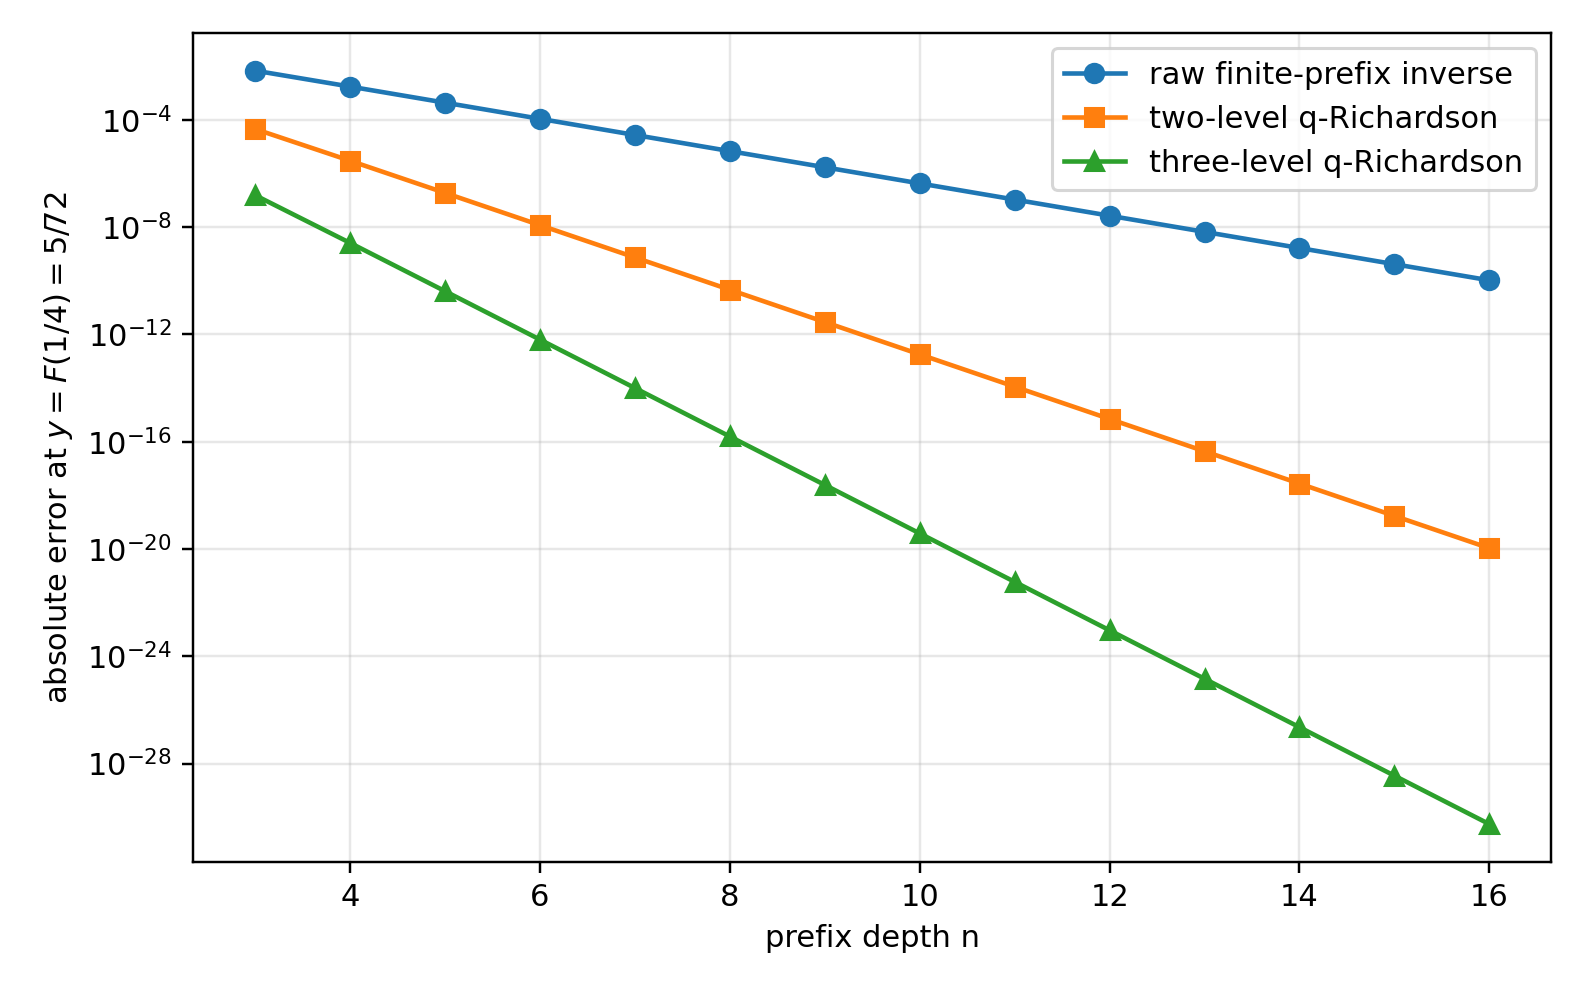
\includegraphics[width=0.92\textwidth]{figures/quarter_quantile_richardson.png}
\caption{Raw and accelerated errors at the exact output $F(1/4)=5/72$.  The
straight-line separation on the logarithmic scale reflects the exact geometric orders
$4^{-n}$, $16^{-n}$, and $64^{-n}$.}
\label{fig:quarter-richardson}
\end{figure}

\subsection{Exact sign and two-sided bounds for every accelerated quarter error}

The preceding asymptotic constants can be strengthened to a finite-$n$ interpolation
statement.  Put
\begin{equation}
 f(Q):=\Delta_2(Q)=\frac{\sqrt{1+(64/9)Q}-1}{8}.
 \label{eq:f-quarter-germ}
\end{equation}
For fixed $n$ and $s$, the quantity
$\mathcal G_{n,s}(5/72)-1/4$ is the value at $Q=0$ of the polynomial of degree
at most $s-1$ interpolating $f$ at the nodes
$4^{-n},4^{-(n+1)},\ldots,4^{-(n+s-1)}$.

\begin{theorem}[Positive accelerated errors and sharp finite-depth bounds]
\label{thm:quarter-positive-bounds}
Let
\begin{equation}
 K_s:=\frac{C_{s-1}2^{-s^2+5s-2}}{9^s}.
 \label{eq:Ks-quarter}
\end{equation}
For every $s\ge1$ and $n\ge3$,
\begin{equation}
 \boxed{
 0< K_s4^{-sn}\left(1+\frac{64}{9}4^{-n}\right)^{\frac12-s}
 <\mathcal G_{n,s}\!\left(\frac5{72}\right)-\frac14
 <K_s4^{-sn}.}
 \label{eq:quarter-two-sided}
\end{equation}
In particular, the ratio of the exact error to its leading term is squeezed to one
inside an explicitly shrinking enclosure.
\end{theorem}

\begin{proof}
Let $p_{n,s-1}$ be the Lagrange interpolant just described.  The interpolation
remainder at zero gives a point $\xi_{n,s}\in(0,4^{-n})$ such that
\begin{equation}
 -p_{n,s-1}(0)
 =\frac{f^{(s)}(\xi_{n,s})}{s!}
   \prod_{j=0}^{s-1}(-4^{-(n+j)}).
 \label{eq:Lagrange-remainder-quarter}
\end{equation}
Now
\begin{equation}
 f^{(s)}(Q)=\frac1{8}\left(\frac12\right)^{\!\underline{s}}
 \left(\frac{64}{9}\right)^s
 \left(1+\frac{64}{9}Q\right)^{\frac12-s},
 \label{eq:f-quarter-derivative}
\end{equation}
where the falling factorial has sign $(-1)^{s-1}$.  The signs in
\eqref{eq:Lagrange-remainder-quarter} therefore imply $p_{n,s-1}(0)>0$.
Using
\begin{equation}
 \frac{\left|\left(\frac12\right)^{\!\underline{s}}\right|}{8s!}
 \left(\frac{64}{9}\right)^s4^{-\binom s2}=K_s
 \label{eq:Ks-identity}
\end{equation}
produces the middle expression in \eqref{eq:quarter-two-sided} with
$\xi_{n,s}$ in place of either endpoint.  Since the exponent $1/2-s$ is
negative, evaluation at $0$ and $4^{-n}$ gives the two strict bounds.
\end{proof}

\begin{remark}
The positivity in \cref{thm:quarter-positive-bounds} is not visible term-by-term in
\eqref{eq:Catalan-qbinom-full}, whose tail alternates.  It is a consequence of the
complete monotonicity pattern of the derivatives of the square-root germ and the sign
of the Lagrange remainder.  This is one concrete place where exact interpolation gives
more information than formal Richardson cancellation.
\end{remark}

\begin{proposition}[Large-order Catalan coefficients]
\label{prop:Catalan-large-order}
The Taylor coefficients of the quarter germ satisfy
\begin{equation}
 \boxed{
 \delta_{2,m}\sim
 (-1)^{m-1}\frac1{16\sqrt\pi}\left(\frac{64}{9}\right)^m m^{-3/2}.}
 \label{eq:Catalan-large-order}
\end{equation}
Thus the branch point $Q=-9/64$ controls both the convergence radius and the
$m^{-3/2}$ algebraic prefactor.
\end{proposition}

\begin{proof}
Insert the classical Catalan asymptotic
$C_{m-1}\sim4^{m-1}/(\sqrt\pi\,m^{3/2})$ into
\eqref{eq:Catalan-germ}.
\end{proof}

\subsection{A universal first coefficient at every inverse-dyadic anchor}

The leading displacement of the algebraic germ admits a particularly compact expression in
the dyadic moment numbers $d_r$ from \eqref{eq:d-def}.

\begin{proposition}[First algebraic-germ coefficient]
\label{prop:first-dyadic-germ-coefficient}
For every $r\ge2$,
\begin{equation}
 \boxed{
 \delta_{r,1}
 =\frac1{18}\frac{F''(2^{-r})}{F'(2^{-r})}
 =\frac{2^{r-1}(r-1)d_{r-2}}{9d_{r-1}}>0.}
 \label{eq:first-dyadic-germ-coefficient}
\end{equation}
For $r=1$, $\Delta_1\equiv0$ and $G_n(1/2)=1/2$ exactly.
\end{proposition}

\begin{proof}
The first equality is \eqref{eq:c1} evaluated at $x_r$.  Formula
\eqref{eq:dyadic-jet} gives
\[
 \frac{F''(x_r)}{F'(x_r)}
 =4\frac{F(2^{2-r})}{F(2^{1-r})}.
\]
Substitute \eqref{eq:d-def} at indices $r-2$ and $r-1$ and simplify the powers
of two.  Positivity follows from $d_j>0$.  The case $r=1$ follows from symmetry
of every prefix density.
\end{proof}

The values $4/9$, $8/5$, and $40/9$ in
\eqref{eq:Catalan-first}, \eqref{eq:Delta3}, and \eqref{eq:Delta4} are therefore
not isolated coincidences; they are the first members of a single exact rational
sequence controlled by adjacent dyadic moments.

\section{Periodic Lambert--Bell inversion at the endpoint}
\label{sec:endpoint-inversion}

\subsection{The forward input and its periodic data}

We now invert the all-orders small-$x$ expansion already established in the corpus.
Put
\begin{equation}
 L:=\log2,
 \qquad B:=1+\frac L2,
 \qquad \beta:=\frac BL=\frac1L+\frac12.
 \label{eq:L-B-beta}
\end{equation}
For sufficiently small $x>0$, the exact lower-Lambert phase is the large positive
solution
\begin{equation}
 x=\lambda2^{-\lambda}=\lambda\e^{-L\lambda},
 \qquad
 \lambda(x)=-\frac1L W_{-1}(-Lx) \cite{CorlessLambertW}.
 \label{eq:exact-lower-Lambert}
\end{equation}
The sharp forward expansion has, for every fixed $N$, the form
\begin{equation}
 \boxed{
 \log F(x)=
 -\frac L2\lambda^2+B\lambda-\frac12\log\lambda
 +C_{\sharp}+\Psi(\lambda)
 +\sum_{j=1}^{N-1}\frac{A_j(\lambda)}{\lambda^j}
 +\bigO_N(\lambda^{-N}).}
 \label{eq:forward-endpoint-all-orders}
\end{equation}
Here every $A_j$ and $\Psi$ is smooth, bounded, and one-periodic.  With
$\gamma$ denoting Euler's constant and $\gamma_1$ the first Stieltjes constant in the
convention
\(
 \zeta(s)=\frac1{s-1}+\sum_{m\ge0}(-1)^m\gamma_m(s-1)^m/m!
\),
\begin{equation}
 C_{\sharp}=
 \frac{6\gamma^2+12\gamma_1-\pi^2}{12L}
 -\frac{7L}{12}-\frac12\log\pi.
 \label{eq:Csharp}
\end{equation}
The zero-mean periodic fluctuation has Fourier coefficients
\begin{equation}
 \Psi(u)=\sum_{k\ne0}\widehat\Psi(k)\e^{2\pi\ii ku},
 \qquad
 \widehat\Psi(k)=-\frac{\Gamma(-\chi_k)\zeta(1-\chi_k)}{L},
 \qquad
 \chi_k=\frac{2\pi\ii k}{L}.
 \label{eq:Psi-Fourier}
\end{equation}
The first logarithmic correction is
\begin{equation}
 \boxed{
 A_1(u)=\frac1{24}+\frac1{2L}
 -\frac{\Psi''(u)+\Psi'(u)^2}{2L^2}.}
 \label{eq:A1-periodic}
\end{equation}
The Gamma factor in \eqref{eq:Psi-Fourier} gives exponential Fourier decay, so all
phase differentiations below are legitimate.

\subsection{Two-scale inversion of the saddle phase}

Let
\begin{equation}
 T:=\log\frac1y,
 \qquad
 \rho:=\sqrt{\frac{2T}{L}},
 \qquad
 \theta:=\rho+\beta.
 \label{eq:T-rho-theta}
\end{equation}
The leading inverse equivalent from the corpus is conveniently written
\begin{equation}
 G_0(y):=\rho\e^{-L\rho-L\beta}
 =\frac{\sqrt T}{\e\sqrt L}\e^{-\sqrt{2LT}}.
 \label{eq:G0}
\end{equation}
The following theorem computes what the corpus left implicit.

\begin{theorem}[Phase inversion through two nontrivial orders]
\label{thm:phase-two-orders}
As $y\downarrow0$, the exact phase of $x=G(y)$ satisfies
\begin{equation}
 \boxed{
 \lambda(G(y))=
 \rho+\beta+\frac{d_1}{\rho}+\frac{d_2}{\rho^2}
 +\bigO\!\left(\frac{(\log\rho)^2}{\rho^3}\right),}
 \label{eq:lambda-inverse-two-orders}
\end{equation}
where all periodic functions below are evaluated at $\theta$ and
\begin{align}
 d_1&=\frac{\beta^2}{2}
 +\frac{C_{\sharp}+\Psi(\theta)-\tfrac12\log\rho}{L},
 \label{eq:d1-endpoint}\\
 d_2&=\frac{\Psi'(\theta)d_1+A_1(\theta)-\tfrac12\beta}{L}.
 \label{eq:d2-endpoint}
\end{align}
Consequently,
\begin{equation}
 \boxed{
 \log\frac{G(y)}{G_0(y)}
 =\frac{h_1}{\rho}+\frac{h_2}{\rho^2}
 +\bigO\!\left(\frac{(\log\rho)^3}{\rho^3}\right),}
 \label{eq:log-inverse-two-orders}
\end{equation}
with
\begin{align}
 h_1&=\beta-Ld_1
 =\frac12\log\rho+\kappa_0-\Psi(\theta),
 \label{eq:h1}\\
 h_2&=d_1-\frac{\beta^2}{2}-Ld_2
 =(1-\Psi'(\theta))d_1-\frac{\beta^2}{2}
   -A_1(\theta)+\frac\beta2,
 \label{eq:h2}\\
 \kappa_0&:=\beta-\frac L2\beta^2-C_{\sharp}
 =\frac1{2L}-\frac L8-C_{\sharp}.
 \label{eq:kappa0}
\end{align}
Equivalently, in multiplicative form,
\begin{equation}
 \boxed{
 \frac{G(y)}{G_0(y)}
 =1+\frac{h_1}{\rho}
 +\frac{h_2+\tfrac12h_1^2}{\rho^2}
 +\bigO\!\left(\frac{(\log\rho)^3}{\rho^3}\right).}
 \label{eq:inverse-multiplicative-two-orders}
\end{equation}
\end{theorem}

\begin{proof}
Negate \eqref{eq:forward-endpoint-all-orders} and use
$T=L\rho^2/2$.  Write
\begin{equation}
 \lambda=\rho+\beta+D,
 \qquad
 D=\frac{d_1}{\rho}+\frac{d_2}{\rho^2}+\cdots.
 \label{eq:lambda-D}
\end{equation}
The quadratic part simplifies exactly:
\begin{equation}
 \frac L2\lambda^2-B\lambda
 =\frac L2\rho^2+L\rho D-\frac L2\beta^2+\frac L2D^2.
 \label{eq:quadratic-cancellation}
\end{equation}
The constant term after cancellation of $L\rho^2/2$ is
\[
 Ld_1-\frac L2\beta^2+\frac12\log\rho-C_{\sharp}-\Psi(\theta),
\]
which gives \eqref{eq:d1-endpoint}.  The coefficient of $\rho^{-1}$ is
\[
 Ld_2+\frac\beta2-\Psi'(\theta)d_1-A_1(\theta),
\]
which gives \eqref{eq:d2-endpoint}.  The all-orders remainder in
\eqref{eq:forward-endpoint-all-orders}, together with $d_1=\bigO(\log\rho)$,
then yields the stated phase remainder by one Newton correction; the derivative of the
phase equation is $L\rho+\bigO(1)$.

Finally,
\begin{align*}
 \log G(y)
 &=\log\lambda-L\lambda\\
 &=\log\rho-L\rho-L\beta
   +\log\!\left(1+\frac\beta\rho+\frac D\rho\right)-LD.
\end{align*}
Expansion through $\rho^{-2}$ gives \eqref{eq:h1}--\eqref{eq:h2}; exponentiation
gives \eqref{eq:inverse-multiplicative-two-orders}.
\end{proof}

The first consequence is the promised explicit correction to the leading equivalent.

\begin{corollary}[First oscillatory relative correction]
\label{cor:first-oscillatory-inverse}
As $y\downarrow0$,
\begin{equation}
 \boxed{
 \frac{G(y)}{G_0(y)}
 =1+\frac{\tfrac12\log\rho+\kappa_0-\Psi(\rho+\beta)}{\rho}
 +\bigO\!\left(\frac{(\log\rho)^2}{\rho^2}\right).}
 \label{eq:first-oscillatory-inverse}
\end{equation}
\end{corollary}

\begin{remark}[Why the exact phase shift matters]
Replacing $\rho+\beta$ by $\rho$, or replacing $\rho$ by a cruder expression in
$\log(1/y)$ inside $\Psi$, changes the phase by a fixed noninteger amount and therefore
changes the correction at its full natural size $1/\rho$.  The constant shift
$\beta=1/L+1/2$ is not optional bookkeeping.
\end{remark}

\subsection{A complete periodic limit set}

The oscillation in \eqref{eq:first-oscillatory-inverse} cannot be absorbed into a
constant second term.

\begin{theorem}[Limit set of the normalized second term]
\label{thm:inverse-limit-set}
Define
\begin{equation}
 \mathscr R(y):=
 \rho\left(\frac{G(y)}{G_0(y)}-1\right)-\frac12\log\rho.
 \label{eq:R-limit-set}
\end{equation}
Then the complete set of subsequential limits as $y\downarrow0$ is
\begin{equation}
 \boxed{
 \range_{y\downarrow0}\mathscr R(y)
 =\bigl[\kappa_0-\max_{u\in[0,1]}\Psi(u),
         \ \kappa_0-\min_{u\in[0,1]}\Psi(u)\bigr].}
 \label{eq:inverse-limit-interval}
\end{equation}
The interval is nondegenerate.  Hence there is no constant $c$ for which
\begin{equation}
 \frac{G(y)}{G_0(y)}
 =1+\frac{\tfrac12\log\rho+c}{\rho}+\smallo(\rho^{-1}).
 \label{eq:no-constant-second-term}
\end{equation}
\end{theorem}

\begin{proof}
Corollary \ref{cor:first-oscillatory-inverse} gives
\begin{equation}
 \mathscr R(y)=\kappa_0-\Psi(\rho+\beta)
 +\bigO\!\left(\frac{(\log\rho)^2}{\rho}\right).
 \label{eq:R-phase}
\end{equation}
As $y$ ranges down to zero, $\rho$ ranges continuously to $+\infty$.  For any
$u\in[0,1)$, choose $\rho_m=m+u-\beta$ and
$y_m=\exp(-L\rho_m^2/2)$.  Then the phase in \eqref{eq:R-phase} is exactly
$u$ modulo one, proving that every value of $\kappa_0-\Psi$ is a subsequential
limit.  Conversely, compactness of the phase circle shows that every sequence has a
phase-convergent subsequence, so no other limit can occur.

The Fourier coefficient $\widehat\Psi(1)$ in \eqref{eq:Psi-Fourier} is nonzero:
Gamma has no zeros and the classical zero-free line $\Re s=1$ gives
$\zeta(1-\chi_1)\ne0$ \cite{TitchmarshZeta}.  Thus $\Psi$ is nonconstant and the interval has positive
length.  Formula \eqref{eq:no-constant-second-term} would force a singleton limit set,
a contradiction.
\end{proof}

\subsection{Quantile elasticity and inverse derivatives}

The logarithmic derivative of the inverse is often more stable numerically than $G'$ itself.

\begin{theorem}[Two-term endpoint elasticity]
\label{thm:quantile-elasticity}
As $y\downarrow0$,
\begin{equation}
 \boxed{
 \frac{yG'(y)}{G(y)}
 =\frac1\rho+\frac{\Psi'(\rho+\beta)-1}{L\rho^2}
 +\bigO\!\left(\frac{\log\rho}{\rho^3}\right).}
 \label{eq:quantile-elasticity}
\end{equation}
Consequently,
\begin{equation}
 G'(y)=\frac{G(y)}{y\rho}
 \left[1+\frac{\Psi'(\rho+\beta)-1}{L\rho}
 +\bigO\!\left(\frac{\log\rho}{\rho^2}\right)\right].
 \label{eq:Gprime-endpoint}
\end{equation}
\end{theorem}

\begin{proof}
Regard both $T=-\log y$ and $\log x$ as functions of the exact phase $\lambda$.
Differentiating \eqref{eq:forward-endpoint-all-orders} gives
\begin{equation}
 \frac{yG'(y)}{G(y)}
 =-\frac{\dd\log x/\dd\lambda}{\dd T/\dd\lambda}
 =\frac{L-\lambda^{-1}}
 {L\lambda-B+\tfrac1{2\lambda}-\Psi'(\lambda)+\bigO(\lambda^{-2})}.
 \label{eq:elasticity-exact-ratio}
\end{equation}
Insert $\lambda=\rho+\beta+\bigO((\log\rho)/\rho)$ and expand.  The terms
containing $\beta$ cancel from the denominator because $B=L\beta$, leaving
\eqref{eq:quantile-elasticity}.
\end{proof}

By reflection, every formula in this section has a right-endpoint counterpart: replace
$y$ by $1-y$ and $G(y)$ by $1-G(y)$.  In particular, the same periodic function and
the same phase shift govern the two ends.

\subsection{An all-orders Lambert--Bell reversion algorithm}

The preceding calculation extends mechanically to every order, but ordinary power-series
notation hides the two-scale nature of the coefficients.  Treat $z=1/\rho$ as the small
variable while holding the fast phase $\theta=\rho+\beta$ and the slow logarithm
$\log\rho$ as coefficient variables.  Let
\begin{equation}
 D(z)=\sum_{m\ge1}d_mz^m,
 \qquad
 \lambda=\rho+\beta+D(z).
 \label{eq:D-formal}
\end{equation}
Define
\begin{align}
 \mathcal R(z,D):={}&-\frac L2\beta^2+\frac L2D^2+\frac12\log\rho
 +\frac12\log(1+\beta z+zD)-C_{\sharp}-\Psi(\theta+D)
 \notag\\
 &-\sum_{j\ge1}A_j(\theta+D)z^j(1+\beta z+zD)^{-j}.
 \label{eq:R-formal-endpoint}
\end{align}
The phase equation is formally
\begin{equation}
 0=\frac LzD+\mathcal R(z,D).
 \label{eq:phase-formal-equation}
\end{equation}

\begin{theorem}[Triangular all-orders endpoint recursion]
\label{thm:all-orders-endpoint-recursion}
Let $D_m(z)=\sum_{j=1}^{m}d_jz^j$ and set $D_0=0$.  The unique formal
solution of \eqref{eq:phase-formal-equation} is generated by
\begin{equation}
 \boxed{
 d_{m+1}=-\frac1L[z^m]\mathcal R(z,D_m),
 \qquad m\ge0.}
 \label{eq:d-all-orders-recursion}
\end{equation}
Each $d_m$ is a polynomial in $\log\rho$ with coefficients in the differential algebra
generated by the periodic functions $\Psi,A_1,\ldots,A_{m-1}$.

Write
\begin{equation}
 \log\frac{G(y)}{G_0(y)}
 =\log(1+\beta z+zD)-LD
 =\sum_{m\ge1}h_mz^m.
 \label{eq:h-all-orders}
\end{equation}
Then the multiplicative coefficients $g_m$ in
\begin{equation}
 \frac{G(y)}{G_0(y)}\sim1+\sum_{m\ge1}g_m\rho^{-m}
 \label{eq:g-all-orders}
\end{equation}
are the complete Bell polynomials
\begin{equation}
 \boxed{
 g_m=\frac1{m!}\mathcal B_m(1!h_1,2!h_2,\ldots,m!h_m).}
 \label{eq:g-Bell}
\end{equation}
For every fixed truncation order, the resulting expansion is rigorous with a remainder
uniform in the phase.
\end{theorem}

\begin{proof}
The coefficient of $d_{m+1}$ in $[z^m](L D/z)$ is exactly $L$, while
$[z^m]\mathcal R$ depends only on $d_1,\ldots,d_m$.  This gives the triangular
recursion.  Taylor expansion of each periodic coefficient at $\theta$ shows inductively
that the coefficient algebra is closed under the required operations.  Formula
\eqref{eq:g-Bell} is the standard exponential formula applied to
\eqref{eq:h-all-orders}.  The uniform all-orders remainder in
\eqref{eq:forward-endpoint-all-orders}, together with the fact that the derivative of the
phase equation is asymptotic to $L\rho$, upgrades the formal induction to a Poincare
expansion at any fixed order.
\end{proof}

\begin{boxedremark}
The endpoint inverse has a mixed asymptotic architecture:
\[
 \text{lower Lambert }W
 \quad+\quad \text{polynomials in }\log\rho
 \quad+\quad \text{periodic Gamma--zeta jets}
 \quad+\quad \text{Bell reversion}.
\]
None of these four layers can be removed without losing a term at some finite order.
\end{boxedremark}

\section{Symbolic, exact, and high-precision verification}
\label{sec:verification}

\subsection{Exact rational checks of the local-polynomial theorem}

The construction of $\mathcal A_r$ was checked independently in exact rational
arithmetic by the following pipeline:
\begin{enumerate}
 \item generate $d_0,\ldots,d_r$ from the recurrence
 \begin{equation}
 d_m=\frac{\sum_{k=0}^{m-1}\binom{m+1}{k}d_k}
 {(m+1)(2^m-1)};
 \label{eq:d-recurrence-check}
 \end{equation}
 \item form the dyadic jet $J_r$ from \eqref{eq:Jr};
 \item generate $b_j$ from \eqref{eq:b-rec};
 \item apply the finite operator in \eqref{eq:Ar-def};
 \item substitute the resulting root series into $\mathcal A_r$ and verify vanishing
 coefficient-by-coefficient.
\end{enumerate}
For $r\le12$, all coefficients through $Q^{12}$ vanish exactly after substitution.
For $r=2$, direct substitution of the radical in \eqref{eq:quarter-exact} reduces the
identity to zero without series expansion.

\subsection{Quarter-anchor convergence and exact enclosures}

\begin{table}[ht]
\centering
\small
\begin{tabular}{@{}r rr rr rr@{}}
\toprule
$n$ & raw error & ratio & $s=2$ error & ratio & $s=3$ error & ratio \\
\midrule
3 & $6.76157\,10^{-3}$ & 0.973666 & $4.51028\,10^{-5}$ & 0.935251 & $1.53350\,10^{-7}$ & 0.915801 \\
4 & $1.72422\,10^{-3}$ & 0.993150 & $2.96269\,10^{-6}$ & 0.982949 & $2.55798\,10^{-9}$ & 0.977675 \\
5 & $4.33277\,10^{-4}$ & 0.998270 & $1.87566\,10^{-7}$ & 0.995679 & $4.06494\,10^{-11}$ & 0.994333 \\
6 & $1.08460\,10^{-4}$ & 0.999566 & $1.17610\,10^{-8}$ & 0.998916 & $6.37859\,10^{-13}$ & 0.998578 \\
7 & $2.71238\,10^{-5}$ & 0.999892 & $7.35660\,10^{-10}$ & 0.999729 & $9.97719\,10^{-15}$ & 0.999644 \\
8 & $6.78150\,10^{-6}$ & 0.999973 & $4.59881\,10^{-11}$ & 0.999932 & $1.55935\,10^{-16}$ & 0.999911 \\
\bottomrule
\end{tabular}
\caption{Exact quarter-quantile errors.  Each ratio divides by the corresponding
leading term in \eqref{eq:quarter-raw-law}--\eqref{eq:quarter-R3-law}.  The values
lie inside the analytic enclosure \eqref{eq:quarter-two-sided}.}
\label{tab:quarter-errors}
\end{table}

The table illustrates a useful distinction.  Richardson acceleration does not merely make
the error small: the exact square-root germ supplies a certified sign and a certified
finite-$n$ relative enclosure.  At $n=8$, three levels already reduce the absolute error
below $1.6\times10^{-16}$.

\subsection{Endpoint inversion on exact dyadic test values}

For $y_n=F(2^{-n})$, the true inverse is exactly $G(y_n)=2^{-n}$.  The dyadic moment
recurrence therefore provides endpoint test values without numerical root finding.  Define
\begin{align}
 G^{[0]}(y)&:=G_0(y),\label{eq:Gapprox0}\\
 G^{[1]}(y)&:=G_0(y)\exp(h_1/\rho),\label{eq:Gapprox1}\\
 G^{[2]}(y)&:=G_0(y)\exp(h_1/\rho+h_2/\rho^2).
 \label{eq:Gapprox2}
\end{align}
The periodic function and its first two derivatives were evaluated from
\eqref{eq:Psi-Fourier} with nine positive Fourier modes at 100 decimal digits.

\begin{table}[ht]
\centering
\small
\begin{tabular}{@{}r r r r r@{}}
\toprule
$n$ & $\rho$ & relative error of $G^{[0]}$ & of $G^{[1]}$ & of $G^{[2]}$ \\
\midrule
5   & 6.43984  & $-3.82510\,10^{-1}$ & $ 7.89489\,10^{-2}$ & $-2.16957\,10^{-2}$ \\
10  & 12.08040 & $-2.56964\,10^{-1}$ & $ 2.68825\,10^{-2}$ & $-4.39948\,10^{-3}$ \\
20  & 22.82438 & $-1.61765\,10^{-1}$ & $ 8.76101\,10^{-3}$ & $-8.23920\,10^{-4}$ \\
40  & 43.65176 & $-9.65552\,10^{-2}$ & $ 2.71602\,10^{-3}$ & $-1.43280\,10^{-4}$ \\
80  & 84.54102 & $-5.53439\,10^{-2}$ & $ 8.04968\,10^{-4}$ & $-2.34032\,10^{-5}$ \\
100 &104.83719 & $-4.59578\,10^{-2}$ & $ 5.39809\,10^{-4}$ & $-1.29189\,10^{-5}$ \\
\bottomrule
\end{tabular}
\caption{Relative errors at the exact points $y_n=F(2^{-n})$.  The first and
second inverse corrections successively remove the dominant endpoint error.}
\label{tab:endpoint-errors}
\end{table}

\begin{figure}[ht]
\centering
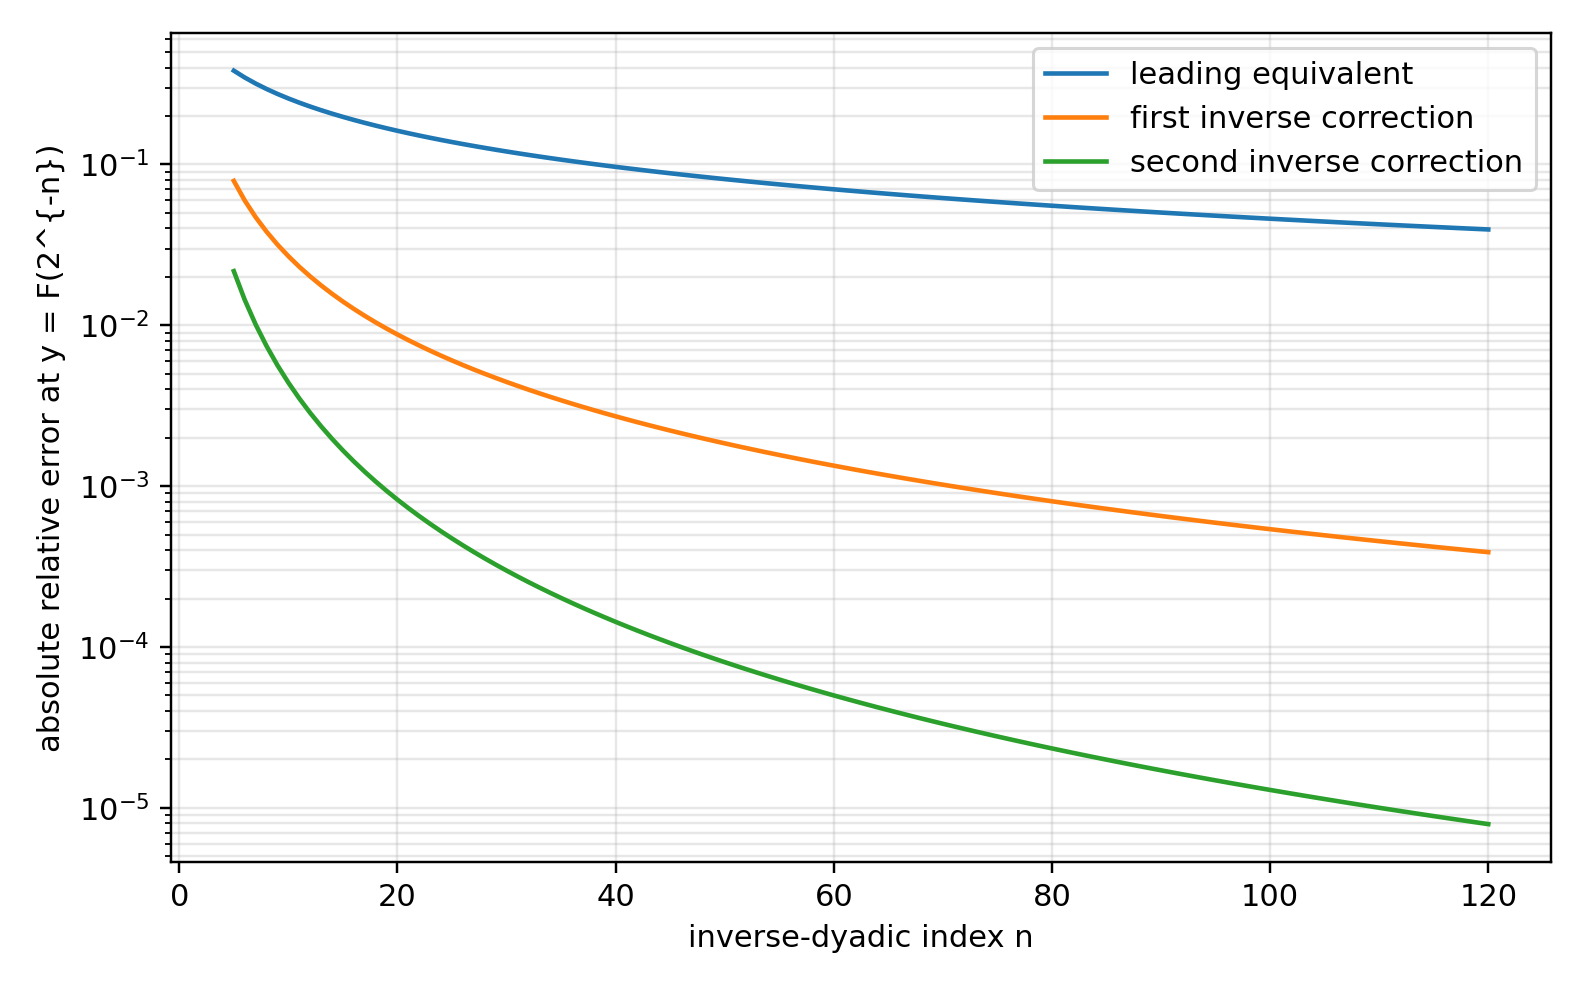
\includegraphics[width=0.92\textwidth]{figures/endpoint_inverse_errors.png}
\caption{Absolute relative errors of the leading, first-corrected, and second-corrected
endpoint inverse approximations on exact inverse-dyadic test values.}
\label{fig:endpoint-errors}
\end{figure}

Numerically,
\begin{equation}
 \begin{split}
 L&=0.6931471805599453094\ldots,\\
 \beta&=1.9426950408889634074\ldots,\\
 C_{\sharp}&=-2.0279838986388594240\ldots,\\
 \kappa_0&=2.6626880215133479640\ldots.
 \end{split}
 \label{eq:endpoint-constants-numeric}
\end{equation}
The first Fourier coefficient has
\begin{equation}
 |\widehat\Psi(1)|=1.0627109779221651\times10^{-6},
 \qquad
 \arg\widehat\Psi(1)=-0.7795055208985225\ldots,
 \label{eq:first-Psi-mode}
\end{equation}
and the second mode is smaller by a factor about $6.30\times10^{-7}$.  Thus $\Psi$ is
very close to a single sinusoid, although its small amplitude does not make it
asymptotically dispensable.

\begin{figure}[ht]
\centering
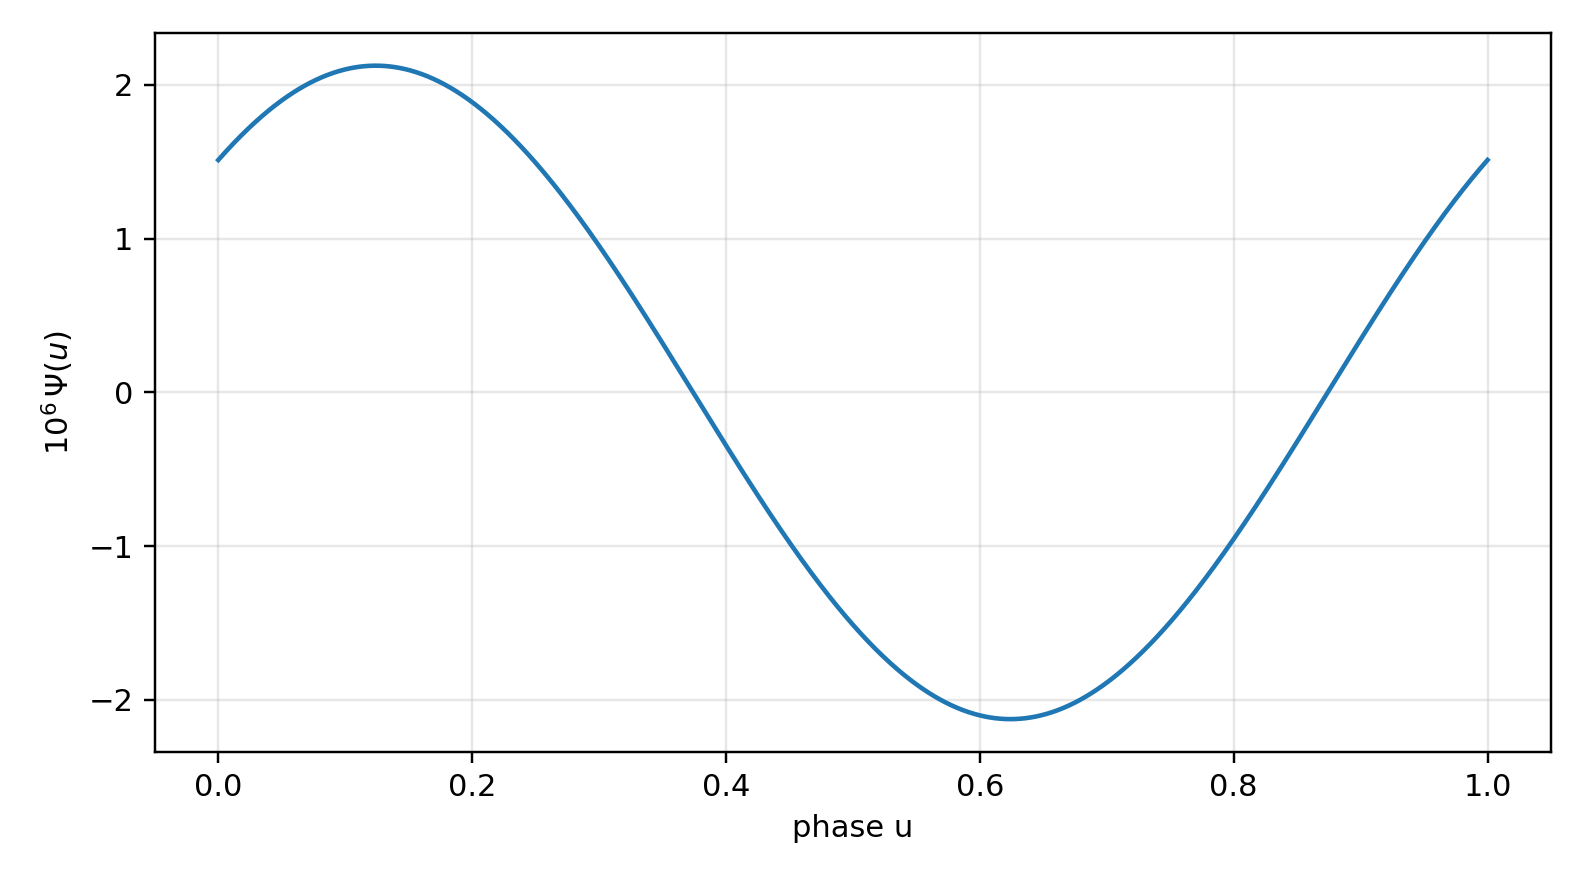
\includegraphics[width=0.92\textwidth]{figures/periodic_inverse_phase.png}
\caption{The periodic Gamma--zeta fluctuation.  The vertical scale is multiplied by
$10^6$.  A grid evaluation gives approximately
$\min\Psi=-2.1254264\times10^{-6}$ and
$\max\Psi=2.1254241\times10^{-6}$.}
\label{fig:Psi-phase}
\end{figure}

The numerical range in \cref{fig:Psi-phase} turns the abstract interval
\eqref{eq:inverse-limit-interval} into an interval of width approximately
$4.25085\times10^{-6}$ centered extremely close to $\kappa_0$.  The width is tiny,
but it is fixed; multiplying the relative error by $\rho$ reveals it rather than erasing it.

\subsection{Independent checks and failure modes}

Three independent representations were used wherever possible:
\begin{enumerate}
 \item exact rational recurrences for $d_r$, $y_r$, $J_r$, and the coefficients of
 $\mathcal A_r$;
 \item symbolic series reversion, including direct residual checks
 $\mathcal A_r(\Delta_r(Q),Q)=\bigO(Q^{M+1})$;
 \item high-precision evaluation of the Gamma--zeta Fourier series and exact dyadic
 inverse test points.
\end{enumerate}
The principal numerical failure mode is phase corruption: replacing the exact
$\theta=\rho+\beta$ by a rounded or asymptotically simplified phase can dominate the
very small periodic signal.  The principal algebraic failure mode is confusing the
forward coefficient $-b_1F''$ with the inverse coefficient $b_1F''/F'$; the missing
Jacobian changes every Richardson constant.

\section{Algorithms and a Lean formalization roadmap}
\label{sec:algorithms-formalization}

\subsection{Exact construction of an inverse-dyadic germ}

The following pseudocode is entirely rational up to the final algebraic root or formal
series operation.

\begin{lstlisting}[style=pseudo,caption={Exact construction of the local polynomial and inverse germ.},label={lst:dyadic-germ}]
input: anchor depth r, requested series order M

# Dyadic moment numbers
D[0] = 1
for m = 1..r:
    D[m] = sum(binomial(m+1,k)*D[k], k=0..m-1)
           / ((m+1)*(2^m-1))

# Reciprocal-sinc coefficients
b[0] = 1
for j = 1..floor(r/2):
    gamma[j] = zeta(2*j)/(j*pi^(2*j)*(4^j-1))  # rational after simplification
    b[j] = sum(k*gamma[k]*b[j-k], k=1..j)/j

# Terminating Fabius jet
J(z) = sum(
    2^(binomial(k+1,2)-binomial(r-k,2))
    * D[r-k] * z^k / (k!*(r-k)!),
    k=1..r)

# Exact finite-prefix local polynomial
A(z,Q) = J(z)
for j = 1..floor(r/2):
    A(z,Q) += (-1)^j * b[j] * Q^j * derivative(J,z,2*j)

# Formal inverse branch A(Delta(Q),Q)=0
Delta(Q) = 0
for m = 1..M:
    residual = coefficient(A(Delta(Q),Q), Q, m)
    delta[m] = -residual / derivative(J,z,1).subs(z=0)
    Delta(Q) += delta[m]*Q^m

return A(z,Q), Delta(Q)
\end{lstlisting}

For $r=2$, a radical solver should be used instead of formal reversion.  For larger $r$,
formal reversion is usually preferable to radicals: it preserves rationality, scales to high
order, and feeds directly into the Gaussian-binomial residual formula.

\subsection{Endpoint coefficient engine}

The all-orders endpoint recursion can be implemented in a differential polynomial ring whose
atoms are $\log\rho$, $\Psi^{(k)}(\theta)$, and $A_j^{(k)}(\theta)$.

\begin{lstlisting}[style=pseudo,caption={Lambert--Bell inverse coefficient engine.},label={lst:endpoint-engine}]
input: desired inverse order N; forward periodic coefficients A[1..N-1]
z = formal variable
D = 0
for m = 0..N-1:
    R = -L*beta^2/2 + L*D^2/2 + log(rho)/2
        + log(1 + beta*z + z*D)/2 - Csharp
        - Taylor_phase(Psi, theta, D)
        - sum(
            Taylor_phase(A[j],theta,D)
            * z^j * (1+beta*z+z*D)^(-j),
            j=1..N-1)
    d[m+1] = -coefficient(R,z,m)/L
    D += d[m+1]*z^(m+1)

H = truncate(log(1+beta*z+z*D)-L*D, z, N)
for m = 1..N:
    h[m] = coefficient(H,z,m)
    g[m] = CompleteBell(m, 1!*h[1], ..., m!*h[m]) / m!
return d, h, g
\end{lstlisting}

The supplied reproducibility script evaluates the first two orders directly rather than
building a general symbolic differential ring, but its formulas are exact transcriptions of
\cref{thm:phase-two-orders}.

\subsection{Formalization modules}

The results separate naturally into five Lean-sized packages.

\begin{obligation}[Polynomial smoothing and inverse moment operator]
Formalize that, for a polynomial $q$ of degree at most $r$,
\[
 M(aD)q=J \quad\Longrightarrow\quad
 q=\sum_{j=0}^{\lfloor r/2\rfloor}(-1)^jb_ja^{2j}D^{2j}J.
\]
This requires only finite sums after the degree bound is known; no convergence theorem for
formal differential operators is needed.
\end{obligation}

\begin{obligation}[Plateau-to-polynomial localization]
Connect the existing almost-everywhere derivative plateau for $p_n^{(r)}$ to the statement
that $p_n$ agrees with a degree-$r$ polynomial on the closed interval
$[\xi_r-2^{-n},\xi_r+2^{-n}]$.  The clean route is repeated absolute continuity of the
spline pieces.
\end{obligation}

\begin{obligation}[Algebraic inverse germ]
Instantiate a formal implicit-function theorem over $\Q[[Q]]$ for
$\mathcal A_r(z,Q)$ with invertible linear coefficient $F'(x_r)$.  Prove separately that
the formal series is represented by the analytic local inverse and enters the plateau interval
for all large $n$.
\end{obligation}

\begin{remark}[Formalized geometric Lagrange core]
The former obligation to formalize \eqref{eq:all-filter-moments} is discharged
at post-snapshot checkpoint
\nolinkurl{1e761ed77583e9870ceeaeb2c74ac824094f0f3f}.  The reusable layer in
\path{CompleteHomogeneous.lean} consists of
\nolinkurl{completeHomogeneousEval_smul},
\nolinkurl{completeHomogeneousEval_option_zero},
\nolinkurl{completeHomogeneousEval_fin_succ},
\nolinkurl{completeHomogeneousEvalOn_range}, and
\nolinkurl{completeHomogeneousEvalAt_zero}.  Over every commutative semiring,
\path{GeometricCompleteHomogeneous.lean} gives
\[
 h_n(1,q,\ldots,q^p)=\qbinom{n+p}{p}{q},
 \qquad
 h_n(c,cq,\ldots,cq^p)=c^n\qbinom{n+p}{p}{q}
\]
through \nolinkurl{completeHomogeneousEval_geometric},
\nolinkurl{completeHomogeneousEval_scaled_geometric}, and the range bridge
\nolinkurl{completeHomogeneousEvalOn_range_pow_eq_gaussianBinomial}.

Over every commutative ring,
\nolinkurl{sum_weight_mul_scaled_geometric_pow_succ_add} and
\nolinkurl{sum_weight_mul_scaled_geometric_pow_of_pos} assume exactness
directly on the nodes \(c q^j\); no nonzero, unit, distinctness, or division
hypothesis is used, even when \(c\) is a zero divisor.  Their unscaled forms
are \nolinkurl{sum_weight_mul_geometric_pow_succ_add} and
\nolinkurl{sum_weight_mul_geometric_pow_of_pos}.  For \(m>0\), the resulting
identity is
\[
 \sum_{j=0}^{p}w_j(cq^j)^m
 =c^m(-1)^p q^{\binom{p+1}{2}}\qbinom{m-1}{p}{q}.
\]
Finite-node injectivity is needed only to instantiate the Lagrange weights in
a field.  The corresponding declarations are
\nolinkurl{sum_geometricLagrangeWeight_mul_pow_succ_add},
\nolinkurl{sum_geometricLagrangeWeight_mul_pow_of_pos},
\nolinkurl{sum_geometricLagrangeWeight_mul_scaled_geometric_pow_of_pos}, and
\nolinkurl{sum_geometricLagrangeWeight_mul_shifted_pow_of_pos}; the last has
the exact \(q\)-exponent
\(start\,m+\binom{p+1}{2}\).  Taking \(p=s-1\), \(c=1\), and \(q=1/4\), after
supplying the elementary finite-node injectivity, gives
\eqref{eq:all-filter-moments} exactly.

This closes only the finite interpolation algebra.  The inverse-germ
substitution, its uniform remainder, and the quarter-error sign/enclosure
theorem---which additionally uses the ordinary Lagrange remainder
sign---remain formalization frontiers.
\end{remark}

\begin{obligation}[Two-scale endpoint reversion]
Build a small asymptotic algebra in the variables $\rho^{-1}$, $\log\rho$, and a phase on
$\R/\Z$.  The first target should be \eqref{eq:first-oscillatory-inverse}; it needs only the
forward expansion through $A_1$ and elementary Taylor bounds.  The all-orders recursion can
then be layered on top of the already formalized forward saddle expansion.
\end{obligation}

The first three remaining obligations are largely algebraic and should be substantially easier
than the existing saddle analysis.  The final two-scale endpoint reversion is analytically
deeper, but the forward uniform remainder estimates already present in the development remove
its most difficult input.

\section{Further deductions and frontier problems}
\label{sec:frontier-problems}

\subsection{Discriminants and convergence radii of the algebraic germs}

For fixed $r$, the radius of convergence of $\Delta_r(Q)$ is bounded by the nearest complex
point where the local branch ceases to be simple.  Algebraically, candidate singularities are
obtained by eliminating $z$ from
\begin{equation}
 \mathcal A_r(z,Q)=0,
 \qquad
 \partial_z\mathcal A_r(z,Q)=0.
 \label{eq:discriminant-system}
\end{equation}
For $r=2$ this gives $Q=-9/64$.  For $r=3$ and $r=4$, the resulting discriminants are
explicit but already nontrivial.  Determining their nearest roots would give exact
large-order laws for $\delta_{r,m}$ and sharp convergence domains for the inverse-prefix
expansions.

\subsection{Validity thresholds}

The proof of \cref{thm:algebraic-germ} yields an unspecified threshold $n_0(r)$ from the
condition $|\Delta_r(4^{-n})|<2^{-n}$.  Computation strongly suggests that the natural
plateau threshold
\begin{equation}
 n\ge r+1
 \label{eq:natural-threshold-conjecture}
\end{equation}
may already suffice for every $r$.  A proof would require a uniform root bound for the small
branch of $\mathcal A_r$ in terms of the positive dyadic moment ratios.  The exact positivity
of \eqref{eq:first-dyadic-germ-coefficient} is encouraging but does not by itself control
higher terms.

\begin{conjecture}[Natural threshold for inverse-dyadic germs]
\label{conj:natural-threshold}
For every $r\ge1$ and every $n\ge r+1$, the small real root
$\Delta_r(4^{-n})$ lies in $[-2^{-n},2^{-n}]$ and
\[
 G_n(F(2^{-r}))=2^{-r}+\Delta_r(4^{-n}).
\]
\end{conjecture}

\subsection{Stieltjes and Bernstein structure}

The quarter germ is a complete Bernstein function of $Q>0$.  This explains the alternating
Catalan coefficients, positivity of every extrapolated error, and the interpolation bounds in
\cref{thm:quarter-positive-bounds}.  It is natural to ask which of the higher algebraic germs
$\Delta_r$ belong to a Stieltjes, Bernstein, or Pick class after an elementary normalization.
A positive answer would turn sign patterns that are currently empirical into global theorems
and might supply Pad\'e bounds stronger than Richardson extrapolation.

\subsection{Uniform transition between finite-prefix and endpoint regimes}

The expansion \eqref{eq:Gn-expansion} is uniform only when the output remains in a compact
subinterval of $(0,1)$, while \cref{sec:endpoint-inversion} treats the exact inverse $G$ as
$y\downarrow0$.  A two-parameter frontier problem is to understand
\begin{equation}
 G_n(y_n)-G(y_n)
 \quad\text{when}\quad y_n\downarrow0
 \label{eq:double-scaling-problem}
\end{equation}
with $n$ simultaneously large.  The crossover should occur when the omitted tail scale
$2^{-n}$ is comparable with the endpoint saddle width.  The exact local polynomial theorem
supplies anchor points inside this transition, and the Lambert phase supplies its natural
continuous coordinate.

\subsection{Optimal phase-aware endpoint approximants}

The first periodic mode of $\Psi$ dominates all later modes by many orders of magnitude.
One may therefore construct inexpensive approximants using only
$\widehat\Psi(\pm1)$ while retaining a rigorous tail bound from Stirling's formula for Gamma
and standard vertical-line estimates for zeta.  A useful computational target is a certified
endpoint inverse routine whose cost is essentially that of evaluating $W_{-1}$ plus one
complex exponential, with a user-prescribed relative error.

\subsection{Inverse functional equations}

The differential identity $F'(x)=2F(2x)$ on the first half of the interval yields
\begin{equation}
 G'(y)=\frac1{2F(2G(y))}
 \qquad (0<y<1/2).
 \label{eq:inverse-functional-derivative}
\end{equation}
The right side can itself be expressed through $G^{-1}$, but not locally in $G(y)$ alone.
A promising direction is to regard the graph of $G$ as an invariant curve for a nonlinear
renormalization operator.  The endpoint expansion in this report gives a formal stable
manifold for that operator, while the inverse-dyadic algebraic germs give exact finite-scale
sections.

\subsection{Publication-priority boundary}

The corpus audit and targeted literature screening found extensive work on arithmetic values,
Fourier products, and dyadic evaluation \cite{AriasArithmetic,Haugland2016}, together with the repository's leading inverse asymptotic, but no occurrence of
the exact local polynomials \eqref{eq:exact-local-Pn}, the Catalan quantile formula
\eqref{eq:quarter-exact}, or the explicit oscillatory inverse correction
\eqref{eq:first-oscillatory-inverse}.  This supports the claim of novelty relative to the
repository and motivates external dissemination.  It does not replace a full bibliographic
priority search, especially across literature using different normalizations of the Fabius or
up-function.

\section{Conclusion}
\label{sec:conclusion}

The Fabius--Rvachev system contains two complementary kinds of self-similarity.  The first is
finite and arithmetic: Thue--Morse inclusion--exclusion, dyadic derivative plateaux, rational
reciprocal-sinc coefficients, and Gaussian $q$-binomial interpolation.  The second is
asymptotic and spectral: lower-Lambert inversion, Gamma--zeta periodicity, and Bell-polynomial
series reversion.  Passing from the function to its inverse makes these structures interact in
ways not visible in the forward theory.

At finite scale, a terminating derivative jet and an exact plateau turn a formal smoothing
inverse into a finite polynomial identity.  This gives algebraic quantile germs at every
inverse-dyadic anchor and, at the quarter anchor, an exact square root with Catalan
coefficients.  Lagrange interpolation on geometric nodes then produces Gaussian-binomial
Richardson laws with closed constants, exact signs, and finite-depth enclosures.

At the endpoint, inverting one additional order beyond the known equivalent reveals the
periodic fluctuation that the leading term suppresses.  Its phase shift is exact, its
subsequential limit set is a nondegenerate interval, and its higher coefficients are generated
by a triangular Lambert--Bell recursion.  The result is a coherent inverse calculus spanning
exact arithmetic, asymptotic analysis, special functions, and extrapolation theory.

\appendix

\section{Complete recursive LaTeX corpus inventory}
\label{app:inventory}

The following ledger records the 57 inspected sources under
\texttt{Analysis/FabiusFunction/docs}.  Historical variants were retained for novelty
screening even when superseded, because they sometimes contain derivations or conjectures not
copied into the living document.

\subsection{Living documents and embedded papers: 25 files}

\begin{longtable}{@{}r p{0.88\textwidth}@{}}
\toprule
No. & Repository-relative path \\
\midrule
\endfirsthead
\toprule
No. & Repository-relative path---continued \\
\midrule
\endhead
1 & \path{FabiusFunction_Mathematical_Glossary/FabiusFunction_Mathematical_Glossary.tex} \\
2 & \path{Fabius_Function_and_Rvachev_Up/Fabius_Function_and_Rvachev_Up.tex} \\
3 & \path{Non_Elementarity_of_the_Fabius_Function/Non_Elementarity_of_the_Fabius_Function.tex} \\
4 & \path{fabius_lean_walkthrough/fabius_lean_walkthrough.tex} \\
5 & \path{non-formalized-research-frontiers/Non_Formalized_Research_Frontiers.tex} \\
6 & \path{non-formalized-research-frontiers/drafts/Fabius_Thue_Morse_Formula_Atlas/Fabius_Thue_Morse_Formula_Atlas.tex} \\
7 & \path{non-formalized-research-frontiers/drafts/rvachev_up_fourier_decay/Rvachev_Up_Fourier_Decay-2/Rvachev_Up_Fourier_Decay.tex} \\
8 & \path{non-formalized-research-frontiers/drafts/rvachev_up_fourier_decay/Rvachev_Up_Fourier_Decay-3/Fourier_decay_of_Rvachev_up.tex} \\
9 & \path{non-formalized-research-frontiers/drafts/rvachev_up_fourier_decay/Rvachev_Up_Fourier_Decay_Comparative_Audit/Rvachev_Up_Fourier_Decay_Comparative_Audit.tex} \\
10 & \path{non-formalized-research-frontiers/drafts/rvachev_up_fourier_decay/Rvachev_Up_Fourier_Decay_Gentle_Guide/Rvachev_Up_Fourier_Decay_Gentle_Guide.tex} \\
11 & \path{non-formalized-research-frontiers/drafts/rvachev_up_fourier_decay/Rvachev_Up_Fourier_Decay_Second_Wave_Audit/Rvachev_Up_Fourier_Decay_Second_Wave_Audit.tex} \\
12 & \path{non-formalized-research-frontiers/drafts/rvachev_up_fourier_decay/asymptotic-decay-rate-of-an-infinite-product-of-sinc-functions/asymptotic-decay-rate-of-an-infinite-product-of-sinc-functions.tex} \\
13 & \path{non-formalized-research-frontiers/drafts/rvachev_up_fourier_decay/rvachev_up_fourier_decay-1/rvachev_up_fourier_decay.tex} \\
14 & \path{non-formalized-research-frontiers/drafts/rvachev_up_fourier_decay/rvachev_up_fourier_decay-4/rvachev_up_fourier_decay.tex} \\
15 & \path{non-formalized-research-frontiers/drafts/rvachev_up_fourier_decay/rvachev_up_fourier_decay-5/Rvachev_Up_Fourier_Decay_Final.tex} \\
16 & \path{non-formalized-research-frontiers/drafts/rvachev_up_fourier_decay/rvachev_up_fourier_decay-6/Rvachev_Up_Fourier_Decay_Final_Synthesis.tex} \\
17 & \path{non-formalized-research-frontiers/drafts/rvachev_up_fourier_decay/rvachev_up_fourier_decay-7/rvachev_up_fourier_decay_final.tex} \\
18 & \path{non-formalized-research-frontiers/drafts/rvachev_up_fourier_decay/rvachev_up_fourier_decay-8/rvachev_up_fourier_decay_final.tex} \\
19 & \path{papers/AIF_2017__67_2_637_0/AIF_2017__67_2_637_0.tex} \\
20 & \path{papers/AIF_2017__67_2_637_0/AIF_2017__67_2_637_0-corrected.tex} \\
21 & \path{papers/arXiv-1502.06738v2/Lacunary_products.tex} \\
22 & \path{papers/arXiv-1702.05442v1/09-Function.tex} \\
23 & \path{papers/arXiv-1702.06487v3/157-Arithmetic-v3.tex} \\
24 & \path{papers/arXiv-2211.13570v1/document.tex} \\
25 & \path{papers/ubiq15/ubiq15-corrected.tex} \\
\bottomrule
\end{longtable}

\subsection{Frozen archive: 32 files}

\begin{longtable}{@{}r p{0.88\textwidth}@{}}
\toprule
No. & Path below \path{archive/} \\
\midrule
\endfirsthead
\toprule
No. & Path below \path{archive/}---continued \\
\midrule
\endhead
1 & \path{early-notes/Fabius Asymptotic/Fabius Asymptotic.tex} \\
2 & \path{early-notes/K-fold summation over the signed Thue-Morse sequence/K-fold summation over the signed Thue-Morse sequence.tex} \\
3 & \path{standalone-studies/Non_Elementarity_of_the_Fabius_Function/Non_Elementarity_of_the_Fabius_Function.tex} \\
4 & \path{standalone-studies/Small_Argument_Asymptotics/Small_Argument_Asymptotics.tex} \\
5 & \path{standalone-studies/fabius-inverse-dyadic-closed-form/fabius-inverse-dyadic-closed-form.tex} \\
6 & \path{primary-exposition/Fabius_Function_and_Rvachev_Up/Fabius_Function_and_Rvachev_Up.tex} \\
7 & \path{primary-exposition/Fabius_Function_and_Rvachev_Up-2/Fabius_Function_and_Rvachev_Up.tex} \\
8 & \path{primary-exposition/Fabius_Function_and_Rvachev_Up-3/Fabius_Function_and_Rvachev_Up.tex} \\
9 & \path{primary-exposition/Fabius_and_Rvachev_Up-2/Fabius_and_Rvachev_Up.tex} \\
10 & \path{primary-exposition/Fabius_and_Rvachev_up/Fabius_and_Rvachev_up.tex} \\
11 & \path{primary-exposition/Fabius_function_and_up_function/Fabius_function_and_up_function.tex} \\
12 & \path{primary-supplements/Fabius_Function_Missing_Parts/Fabius_Function_Missing_Parts.tex} \\
13 & \path{primary-supplements/Fabius_Function_Missing_Parts-2/Fabius_Function_Missing_Parts.tex} \\
14 & \path{q-calculus/Fabius_q_Special_Functions/Fabius_q_Special_Functions.tex} \\
15 & \path{q-calculus/fabius-q-special-functions/fabius-q-special-functions.tex} \\
16 & \path{lean-walkthrough/fabius_lean_walkthrough/fabius_lean_walkthrough.tex} \\
17 & \path{lean-walkthrough/fabius_lean_walkthrough-2/fabius_lean_walkthrough.tex} \\
18 & \path{glossary/FabiusFunction_Mathematical_Glossary/FabiusFunction_Mathematical_Glossary.tex} \\
19 & \path{glossary/FabiusFunction_Mathematical_Glossary-2/FabiusFunction_Mathematical_Glossary.tex} \\
20 & \path{research-frontiers/Fabius_Dyadic_Asymptotic_Bridge/Fabius_Dyadic_Asymptotic_Bridge.tex} \\
21 & \path{research-frontiers/Fabius_Dyadic_Formulae_and_Alternative_Representations/Fabius_Dyadic_Formulae_and_Alternative_Representations.tex} \\
22 & \path{research-frontiers/Fabius_Dyadic_Formulae_to_Asymptotics/Fabius_Dyadic_Formulae_to_Asymptotics.tex} \\
23 & \path{research-frontiers/Fabius_Dyadic_q_Connections/Fabius_Dyadic_q_Connections.tex} \\
24 & \path{research-frontiers/Fabius_Thue_Morse_Convergence_Rate/Fabius_Thue_Morse_Convergence_Rate.tex} \\
25 & \path{research-frontiers/Fabius_Thue_Morse_Convergence_Rates/Fabius_Thue_Morse_Convergence_Rates.tex} \\
26 & \path{research-frontiers/Primary_Exposition_Gap_Register/Primary_Exposition_Gap_Register.tex} \\
27 & \path{research-frontiers/Repeated_Integration_and_Rvachev_Up/Repeated_Integration_and_Rvachev_Up.tex} \\
28 & \path{research-frontiers/Rvachev_Up_from_Repeated_Integration/Rvachev_Up_from_Repeated_Integration.tex} \\
29 & \path{research-frontiers/non-formalized-research-frontiers/non-formalized-research-frontiers.tex} \\
30 & \path{research-frontiers/Thue_Morse_Formula_Atlas-1/Thue_Morse_Formula_Atlas.tex} \\
31 & \path{research-frontiers/Thue_Morse_Formula_Atlas-2/Consolidated_Formula_Atlas_for_the_Thue_Morse_Sequence.tex} \\
32 & \path{research-frontiers/Thue_Morse_Formula_Atlas-3/Thue_Morse_Formula_Atlas.tex} \\
\bottomrule
\end{longtable}

\section{Compact coefficient reference}
\label{app:coefficients}

\subsection{Reciprocal-sinc coefficients}

With $\gamma_j$ from \eqref{eq:gamma-def},
\begin{equation}
 b_0=1,
 \qquad
 b_m=\frac1m\sum_{j=1}^{m}j\gamma_jb_{m-j}.
 \label{eq:b-reference-rec}
\end{equation}
The first values are repeated here for computation:
\begin{equation}
 \begin{array}{c|ccccc}
 m&0&1&2&3&4\\ \hline
 b_m&1&\dfrac1{18}&\dfrac{31}{16200}&
 \dfrac{2347}{42865200}&\dfrac{1904369}{1311675120000}
 \end{array}
 \label{eq:b-reference-table}
\end{equation}

\subsection{Inverse-transfer coefficients}

For a general forward germ
$P_Q(x)=F(x)+\sum_{j\ge1}a_j(x)Q^j$ and inverse
$G_Q(y)=G(y)+\sum_{j\ge1}c_j(y)Q^j$, evaluated at $x=G(y)$,
\begin{align}
 c_1&=-\frac{a_1}{F'},
 \label{eq:c1-general-ref}\\
 c_2&=-\frac{a_2+a_1'c_1+\tfrac12F''c_1^2}{F'},
 \label{eq:c2-general-ref}\\
 c_3&=-\frac{1}{F'}\left(
 a_3+a_2'c_1+a_1'c_2+\frac12a_1''c_1^2
 +F''c_1c_2+\frac16F'''c_1^3\right).
 \label{eq:c3-general-ref}
\end{align}
These are the first rows of the Bell recursion \eqref{eq:Bell-inverse-recursion}.

\subsection{Endpoint reference}

For $T=\log(1/y)$,
\begin{equation}
 \rho=\sqrt{\frac{2T}{L}},
 \qquad
 \theta=\rho+\frac1L+\frac12,
 \qquad
 G_0=\frac{\sqrt T}{\e\sqrt L}\e^{-\sqrt{2LT}}.
 \label{eq:endpoint-reference-vars}
\end{equation}
The first two log-corrections are
\begin{align}
 h_1&=\frac12\log\rho+\kappa_0-\Psi(\theta),
 \label{eq:h1-reference}\\
 h_2&=(1-\Psi'(\theta))
 \left[\frac{\beta^2}{2}+\frac{C_{\sharp}+\Psi(\theta)-\tfrac12\log\rho}{L}\right]
 -\frac{\beta^2}{2}-A_1(\theta)+\frac\beta2.
 \label{eq:h2-reference}
\end{align}
Then $G\approx G_0\exp(h_1/\rho+h_2/\rho^2)$.

\section{Reproducibility files}
\label{app:reproducibility}

The archive accompanying this report contains:
\begin{itemize}
 \item the present LaTeX source and compiled PDF;
 \item the three plotted PNG figures;
 \item \path{generate_data.py}, using exact Python fractions, \texttt{mpmath}, and
 \texttt{matplotlib};
 \item CSV tables for the exact quarter errors and high-precision endpoint tests;
 \item a text file recording the numerical constants and sampled periodic extrema.
\end{itemize}
The Python script makes no network requests.  Re-running it regenerates every numerical
value and figure used in \cref{sec:verification}.

\begin{thebibliography}{99}

\bibitem{Fabius1966}
J.~Fabius,
\newblock A probabilistic example of a nowhere analytic $C^\infty$-function,
\newblock \emph{Zeitschrift f\"ur Wahrscheinlichkeitstheorie und Verwandte
Gebiete} \textbf{5} (1966), 173--174.

\bibitem{Rvachev1990}
V.~A.~Rvachev,
\newblock Compactly supported solutions of functional-differential equations and their
applications,
\newblock \emph{Russian Mathematical Surveys} \textbf{45} (1990), no.~1, 87--120.

\bibitem{Arias1982}
J.~Arias de Reyna,
\newblock Definici\'on y estudio de una funci\'on indefinidamente diferenciable de soporte
compacto,
\newblock \emph{Revista de la Real Academia de Ciencias Exactas, F\'isicas y Naturales de
Madrid} \textbf{76} (1982), no.~1, 21--38;
English translation, arXiv:1702.05442 (2017).

\bibitem{AriasArithmetic}
J.~Arias de Reyna,
\newblock Arithmetic of the Fabius function,
\newblock \emph{INTEGERS} \textbf{18} (2018), Article A51;
arXiv:1702.06487.

\bibitem{Haugland2016}
J.~K.~Haugland,
\newblock Evaluating the Fabius function,
\newblock arXiv:1609.07999 (2016).

\bibitem{AlloucheShallit}
J.-P.~Allouche and J.~Shallit,
\newblock \emph{Automatic Sequences: Theory, Applications, Generalizations},
\newblock Cambridge University Press, 2003.

\bibitem{GasperRahman}
G.~Gasper and M.~Rahman,
\newblock \emph{Basic Hypergeometric Series}, second edition,
\newblock Cambridge University Press, 2004.

\bibitem{AndrewsPartitions}
G.~E.~Andrews,
\newblock \emph{The Theory of Partitions},
\newblock Addison--Wesley, 1976.

\bibitem{CorlessLambertW}
R.~M.~Corless, G.~H.~Gonnet, D.~E.~G.~Hare, D.~J.~Jeffrey, and D.~E.~Knuth,
\newblock On the Lambert $W$ function,
\newblock \emph{Advances in Computational Mathematics} \textbf{5} (1996), 329--359.

\bibitem{Comtet}
L.~Comtet,
\newblock \emph{Advanced Combinatorics: The Art of Finite and Infinite Expansions},
\newblock D.~Reidel, 1974.

\bibitem{deBoorSplines}
C.~de Boor, K.~H\"ollig, and S.~Riemenschneider,
\newblock \emph{Box Splines},
\newblock Springer, 1993.

\bibitem{TitchmarshZeta}
E.~C.~Titchmarsh,
\newblock \emph{The Theory of the Riemann Zeta-Function}, second edition, revised by
D.~R.~Heath-Brown,
\newblock Oxford University Press, 1986.

\bibitem{DLMF}
NIST Digital Library of Mathematical Functions,
\newblock Chapters 4, 17, 24, and 26: Lambert $W$, $q$-hypergeometric functions,
Bernoulli polynomials, and combinatorial analysis,
\newblock \url{https://dlmf.nist.gov/}.

\bibitem{ProveItPrimary}
V.~Reshetnikov,
\newblock \emph{The Fabius Function and Rvachev's Up Function: Self-similarity,
probability, exact dyadic arithmetic, and the corrected small-argument asymptotic},
\newblock living manuscript in the \texttt{ProveIt} repository, 2026,
\newblock \url{https://github.com/VladimirReshetnikov/ProveIt/blob/main/Analysis/FabiusFunction/docs/Fabius_Function_and_Rvachev_Up/Fabius_Function_and_Rvachev_Up.tex}.

\bibitem{ProveItMissing}
V.~Reshetnikov,
\newblock \emph{Fabius Function---Missing Parts},
\newblock repository manuscript, 2026.

\bibitem{ProveItAtlas}
V.~Reshetnikov,
\newblock \emph{A Unified Formula Atlas for the Thue--Morse Sequence},
\newblock repository manuscript, 2026.

\bibitem{ProveItFrontiers}
V.~Reshetnikov,
\newblock \emph{Non-Formalized Research Frontiers for the Fabius Function},
\newblock repository manuscript, 2026.

\bibitem{ProveItFourier}
V.~Reshetnikov,
\newblock \emph{The Fourier Decay of Rvachev's Up-Function: Final Resolution},
\newblock repository manuscript, 2026.

\end{thebibliography}

\end{document}
